\documentclass[12pt,a4paper]{article}

% ── Core packages (all part of standard texlive-latex-recommended) ─────────────
\usepackage[margin=2.5cm]{geometry}
\setlength{\headheight}{14pt}
\usepackage{graphicx}
\usepackage{booktabs}
\usepackage{array}
\usepackage{amsmath}
\usepackage{amssymb}
\usepackage{hyperref}
\usepackage{xcolor}
\usepackage{caption}
\usepackage{float}
\usepackage{multirow}
\usepackage{fancyhdr}
\usepackage{parskip}       % paragraph spacing instead of indent

% ── Colours ───────────────────────────────────────────────────────────────────
\definecolor{hpcblue}{RGB}{44,123,182}
\definecolor{lightgray}{RGB}{245,245,245}
\definecolor{midgray}{RGB}{180,180,180}
\definecolor{darkgreen}{RGB}{0,128,0}

% ── Header / Footer ───────────────────────────────────────────────────────────
\pagestyle{fancy}
\fancyhf{}
\rhead{\small EC7207 --- High Performance Computing}
\lhead{\small Group 11 --- Analysis Report}
\cfoot{\thepage}
\renewcommand{\headrulewidth}{0.4pt}

% ── Hyperlinks ─────────────────────────────────────────────────────────────────
\hypersetup{colorlinks=true, linkcolor=hpcblue, urlcolor=hpcblue}

% ── Column types ──────────────────────────────────────────────────────────────
\newcolumntype{C}[1]{>{\centering\arraybackslash}p{#1}}
\newcolumntype{L}[1]{>{\raggedright\arraybackslash}p{#1}}
\newcolumntype{R}[1]{>{\raggedleft\arraybackslash}p{#1}}

% ── Verbatim-style inline code ─────────────────────────────────────────────────
\newcommand{\code}[1]{\texttt{\small #1}}

% ─────────────────────────────────────────────────────────────────────────────
\begin{document}

% ══════════════════════════════════════════════════════════════════════════════
% TITLE PAGE
% ══════════════════════════════════════════════════════════════════════════════
\begin{titlepage}
\centering
\vspace*{2cm}

{\large EC7207: High Performance Computing\\[0.5em]}
{\large Analysis Report\\[2em]}

\noindent\rule{\linewidth}{1.5pt}\\[0.6em]
{\Huge\bfseries\color{hpcblue}
  Parallel Pearson Correlation\\[0.3em]
  Based Recommendation System\\[0.6em]
}
\noindent\rule{\linewidth}{1.5pt}\\[2em]

{\large\bfseries Group Number: 11\\[1em]}
{
  EG/2021/4417 \quad Ashfaq M.R.M.\\[0.4em]
  EG/2021/4419 \quad Athanayaka K.A.L.G.\\[0.4em]
  EG/2021/4424 \quad Balasooriya J.M.\\[2.5em]
}

{\small Technologies: Serial (C) $\cdot$ OpenMP $\cdot$ Pthreads $\cdot$ MPI $\cdot$ CUDA $\cdot$ Hybrid MPI+OpenMP\\[0.3em]
Problem: 1\,000 users $\times$ 1\,000 items $\cdot$ SEED=42 $\cdot$ Sparsity=70\% $\cdot$ TOP-K=20\\[0.3em]
Platform: Pop!\_OS 24.04 LTS $\cdot$ GCC 13.3.0 $\cdot$ Open MPI 4.1.6 $\cdot$ CUDA 12.0\\[0.2em]
Intel Core i7-11800H (8 physical / 16 logical cores) $\cdot$ NVIDIA GeForce RTX 3050 Laptop GPU\\[2em]
May 2026}

\end{titlepage}

\tableofcontents
\newpage

% ══════════════════════════════════════════════════════════════════════════════
\section{Introduction}
% ══════════════════════════════════════════════════════════════════════════════

Modern collaborative filtering recommendation systems compute pairwise user
similarity over large rating matrices.  For $N = M = 1{,}000$ users and items,
this amounts to 499\,500 Pearson pair computations totalling approximately
500 million floating-point operations --- the dominant bottleneck.

This report documents the implementation and performance evaluation of a
\textbf{Pearson Correlation-Based Collaborative Filtering Recommender System}
parallelised with OpenMP, POSIX Threads (Pthreads), MPI, CUDA, and Hybrid
MPI+OpenMP.  All versions are benchmarked on a single Linux machine
(Intel Core i7-11800H, 8 physical / 16 logical cores) with an NVIDIA GeForce
RTX 3050 Laptop GPU for the CUDA version (see Section~\ref{sec:cuda-results}).

\subsection*{Experimental Configuration}

\begin{table}[H]
\centering
\begin{tabular}{l L{8.7cm}}
\toprule
\textbf{Parameter}     & \textbf{Value} \\
\midrule
Users ($N$)            & 1\,000 \\
Items ($M$)            & 1\,000 \\
Sparsity               & 70\% \\
Test split             & 10\%  \quad (29\,866 held-out ratings) \\
TOP-K neighbours       & 20 \\
Random seed            & 42 \\
Benchmark thread/process counts & 1, 2, 4, 8 \\
Timing method          & \code{clock\_gettime} / \code{omp\_get\_wtime} / \code{MPI\_Wtime} / \code{cudaEvent} (GPU) \\
Platform               & Pop!\_OS 24.04 LTS, GCC 13.3.0, Open MPI 4.1.6, CUDA 12.0 \\
CPU / GPU              & Intel Core i7-11800H (8 phys / 16 logical) / NVIDIA RTX 3050 Laptop GPU \\
\bottomrule
\end{tabular}
\caption{Fixed benchmark parameters used across all versions.}
\end{table}

% ══════════════════════════════════════════════════════════════════════════════
\section{Algorithm Design and Parallel Programming Concepts}
% ══════════════════════════════════════════════════════════════════════════════

\subsection{Algorithm Pipeline (5 Phases)}

\begin{table}[H]
\centering
\begin{tabular}{C{1.2cm} L{3cm} L{6.5cm} L{3.5cm}}
\toprule
\textbf{Phase} & \textbf{Name} & \textbf{Description} & \textbf{Complexity} \\
\midrule
1 & Data Generation  & Synthetic sparse matrix; 10\% test split & $O(N \times M)$ \\
2 & User Means       & Per-user mean $\mu_u$                   & $O(N \times M)$ \\
3 & Similarity       & Pearson for all $(u,v)$ pairs --- bottleneck & $O(N^2 \times M)$ \\
4 & Predictions      & TOP-K weighted prediction               & $O(N^2 \times M)$ \\
5 & MAE Evaluation   & Error on held-out test set              & $O(|T|)$ \\
\bottomrule
\end{tabular}
\caption{Algorithm phases and computational complexity.}
\end{table}

\textbf{Pearson correlation (Phase 3):}
\[
  \text{sim}(u,v) = \frac{\sum_i (R_{ui}-\mu_u)(R_{vi}-\mu_v)}
    {\sqrt{\sum_i (R_{ui}-\mu_u)^2}\;\sqrt{\sum_i (R_{vi}-\mu_v)^2}}
\]

\textbf{Prediction formula (Phase 4):}
\[
  \hat{r}_{ui} = \mu_u + \frac{\sum_{k \in N_K(u)} \text{sim}(u,k)\,(R_{ki}-\mu_k)}
                              {\sum_{k \in N_K(u)} \text{sim}(u,k)}
\]

Both phases are \emph{embarrassingly parallel at the row level}, making them
ideal targets for all five parallelisation strategies.

\begin{figure}[H]
  \centering
  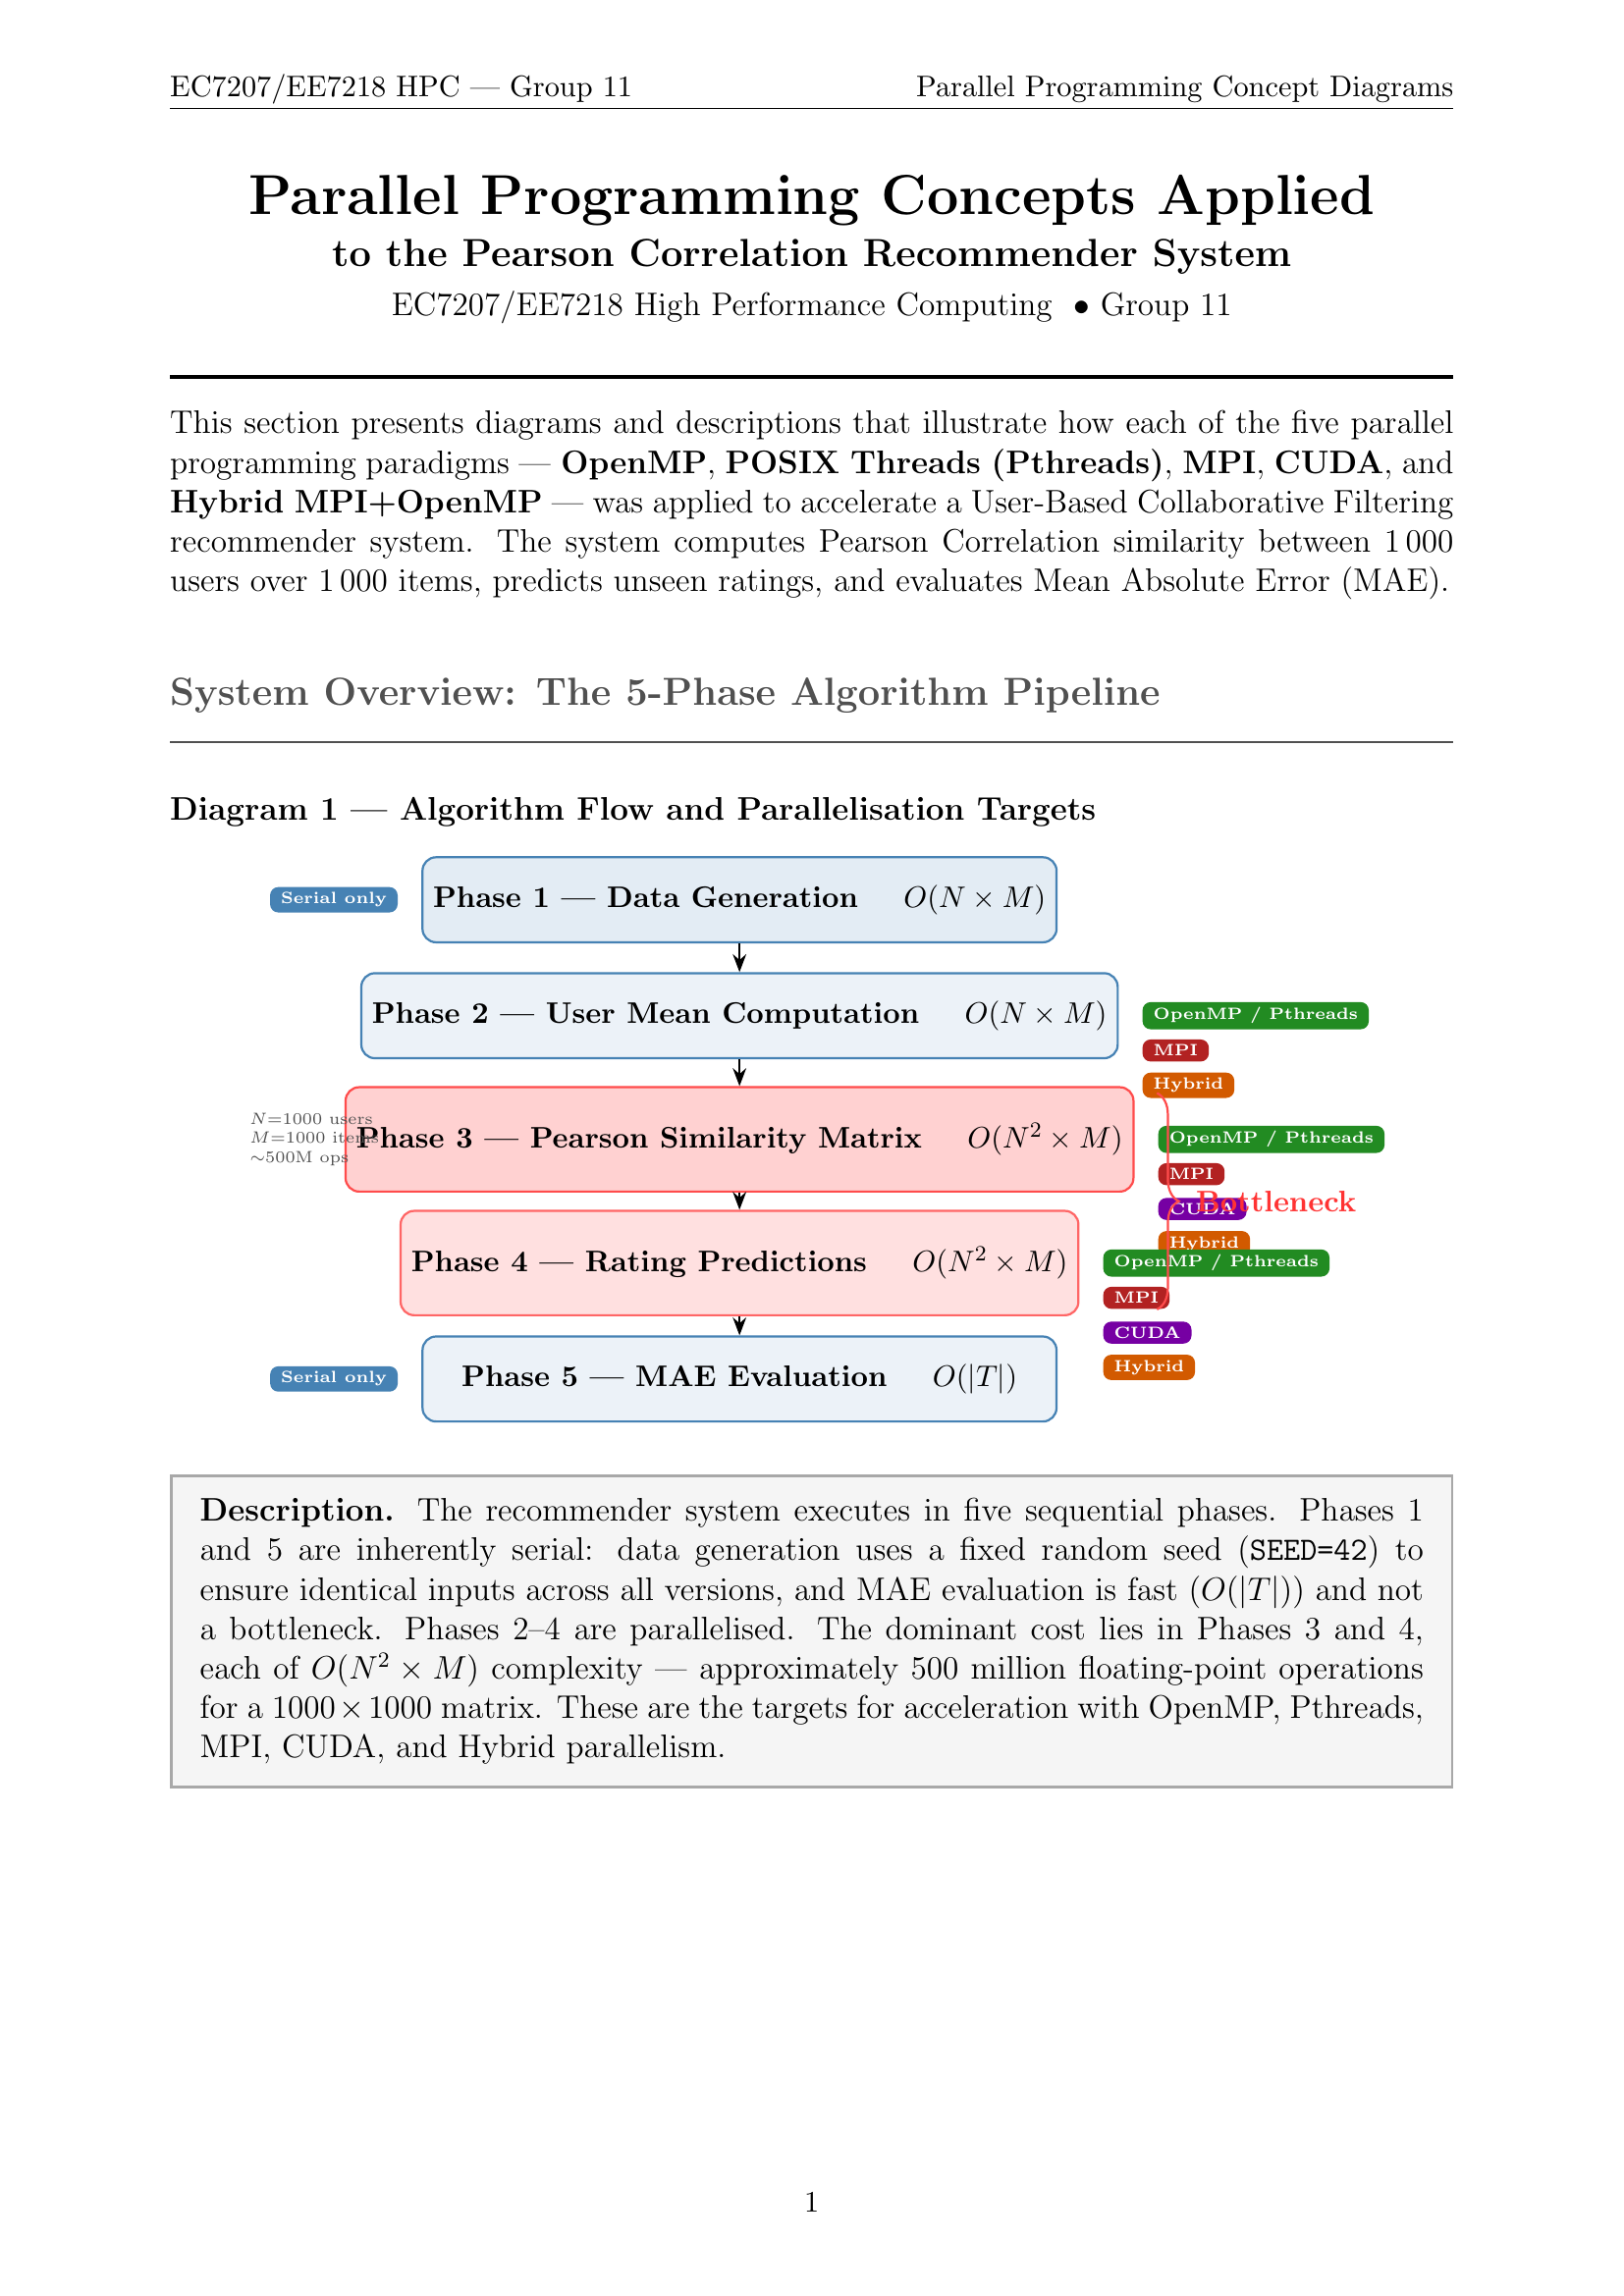
\includegraphics[width=0.92\textwidth]{../analysis_diagrams/charts/concept_overview.png}
  \caption{How the parallel programming concepts map onto the recommender
  pipeline. Phases 3 (similarity) and 4 (prediction) dominate the runtime and
  are partitioned by user-row across every parallel model.}
\end{figure}

\begin{figure}[H]
  \centering
  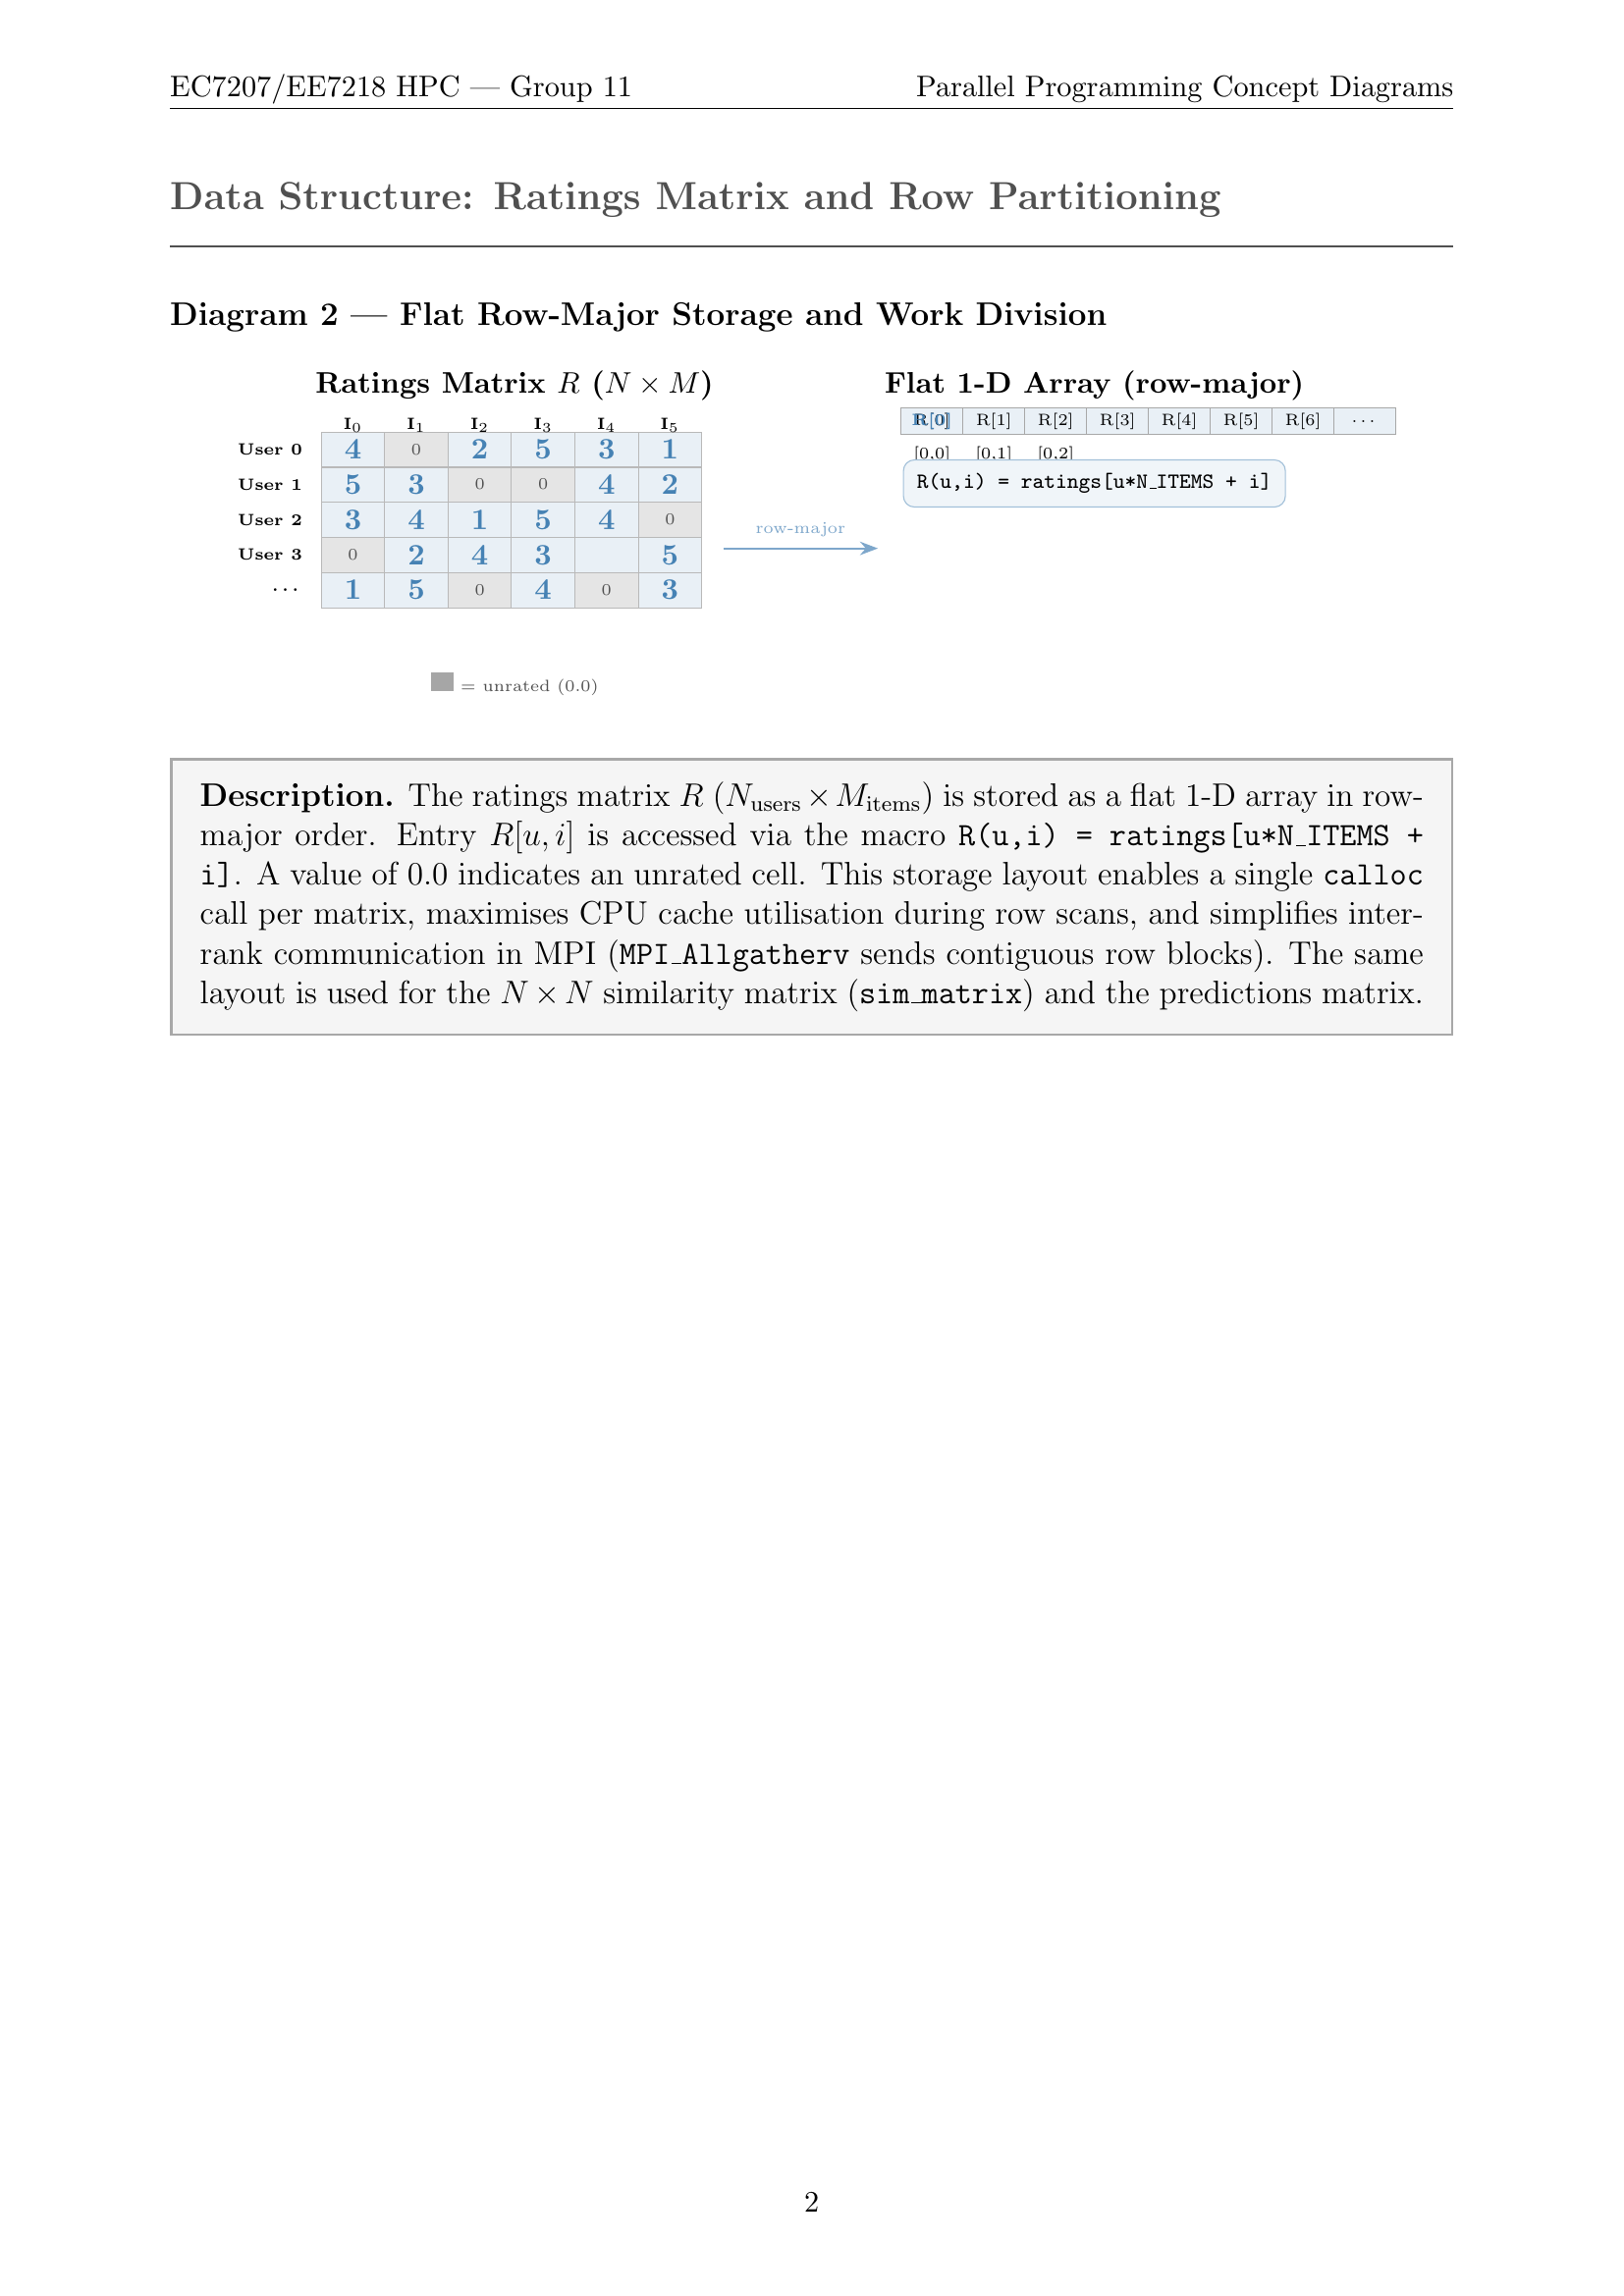
\includegraphics[width=0.78\textwidth]{../analysis_diagrams/charts/concept_partition.png}
  \caption{Row-wise domain decomposition of the ratings/similarity matrices.
  Each worker (OpenMP thread, Pthread, MPI rank, or CUDA thread) owns a disjoint
  set of user rows~$u$ and writes only those rows --- the key to race-freedom.}
\end{figure}

% ─────────────────────────────────────────────────────────────────────────────
\subsection{OpenMP --- Shared-Memory Fork-Join Parallelism}

OpenMP exploits shared-memory parallelism using compiler directives.
A master thread forks into $T$ workers sharing the same address space,
then rejoins at an implicit barrier.

\textbf{Phase 3 (key design choice):}
The outer loop uses \code{\#pragma omp parallel for schedule(dynamic,4)}.
Dynamic scheduling is essential because the triangular loop creates severe load
imbalance: thread 0 processes $N{-}1 = 999$ Pearson calls while the last thread
processes~1.  Dynamic scheduling lets idle threads pull 4-row chunks from a
shared work queue, eliminating wasted CPU time.

\textbf{Race-freedom:}  Each thread owns an exclusive set of outer-loop rows~$u$
and writes \code{SIM(u,v)} only for those rows.  No two threads write the same
cell; no mutex is required.

\textbf{Phase 5 (MAE/RMSE):}  The \code{reduction(+:err)} clause gives each thread
a private accumulator; OpenMP sums all copies at the barrier.  The same pattern
(\code{reduction(+:sq)}) accumulates squared error for RMSE.

\begin{figure}[H]
  \centering
  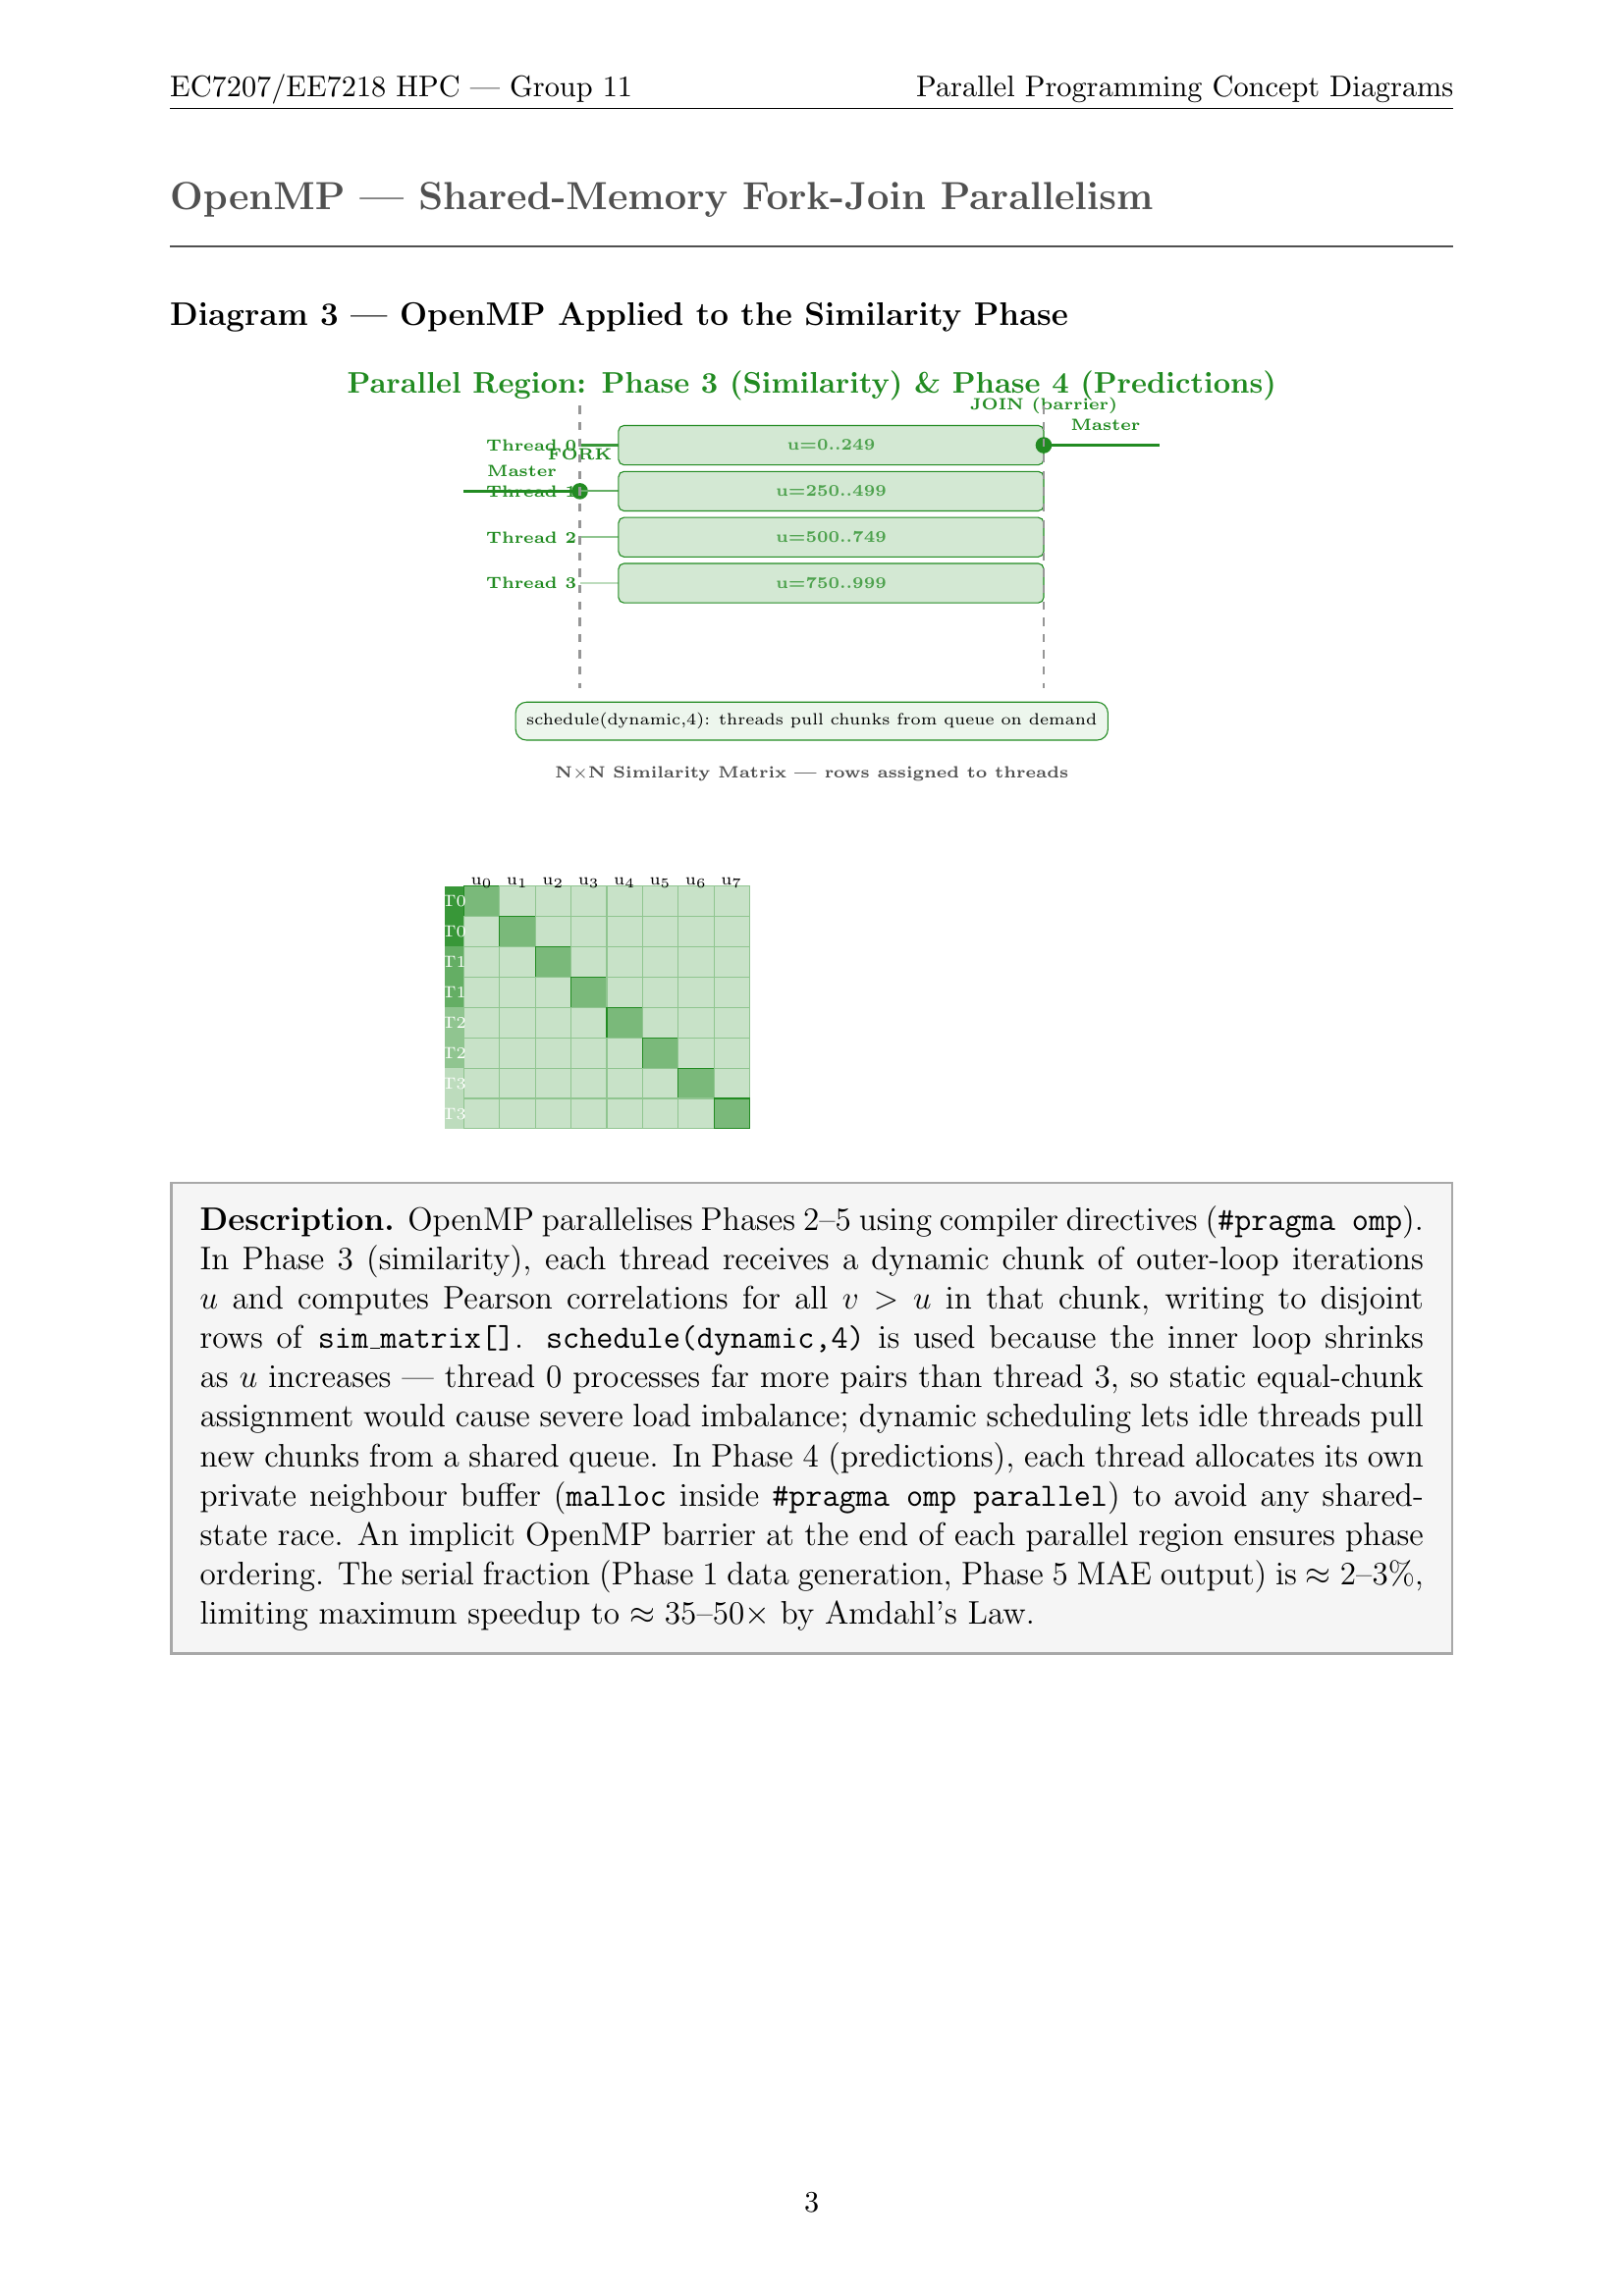
\includegraphics[width=0.85\textwidth]{../analysis_diagrams/charts/concept_openmp.png}
  \caption{OpenMP fork-join model applied to Phases 3--4. A master thread forks
  $T$ workers that pull dynamic row-chunks from a shared queue, then rejoin at an
  implicit barrier.}
\end{figure}

% ─────────────────────────────────────────────────────────────────────────────
\subsection{Pthreads --- Manual POSIX Thread Management}

POSIX Threads require the programmer to explicitly create threads, assign work,
and synchronise with \code{pthread\_join}.

A \code{run\_parallel(fn, nthreads)} harness is called at the start of each of
Phases 2, 3, and 4:
\begin{enumerate}
  \item \code{pthread\_create()} creates $T$ threads, each receiving a
        \code{ThreadArgs} struct with its \code{tid} and total \code{nthreads}.
  \item Each thread derives its exclusive row range:
        $\text{start} = tid \times \lceil N/T \rceil$,
        $\text{end} = \min(\text{start}+\lceil N/T\rceil,\,N)$.
  \item \code{pthread\_join()} acts as a phase barrier.
\end{enumerate}

\textbf{Key difference from OpenMP:}  Threads are created and joined three
separate times (once per phase), paying OS thread-creation overhead three
times per run.  Static row assignment also cannot compensate for the triangular
loop imbalance --- which explains the slightly lower efficiency vs.\ OpenMP.

\begin{figure}[H]
  \centering
  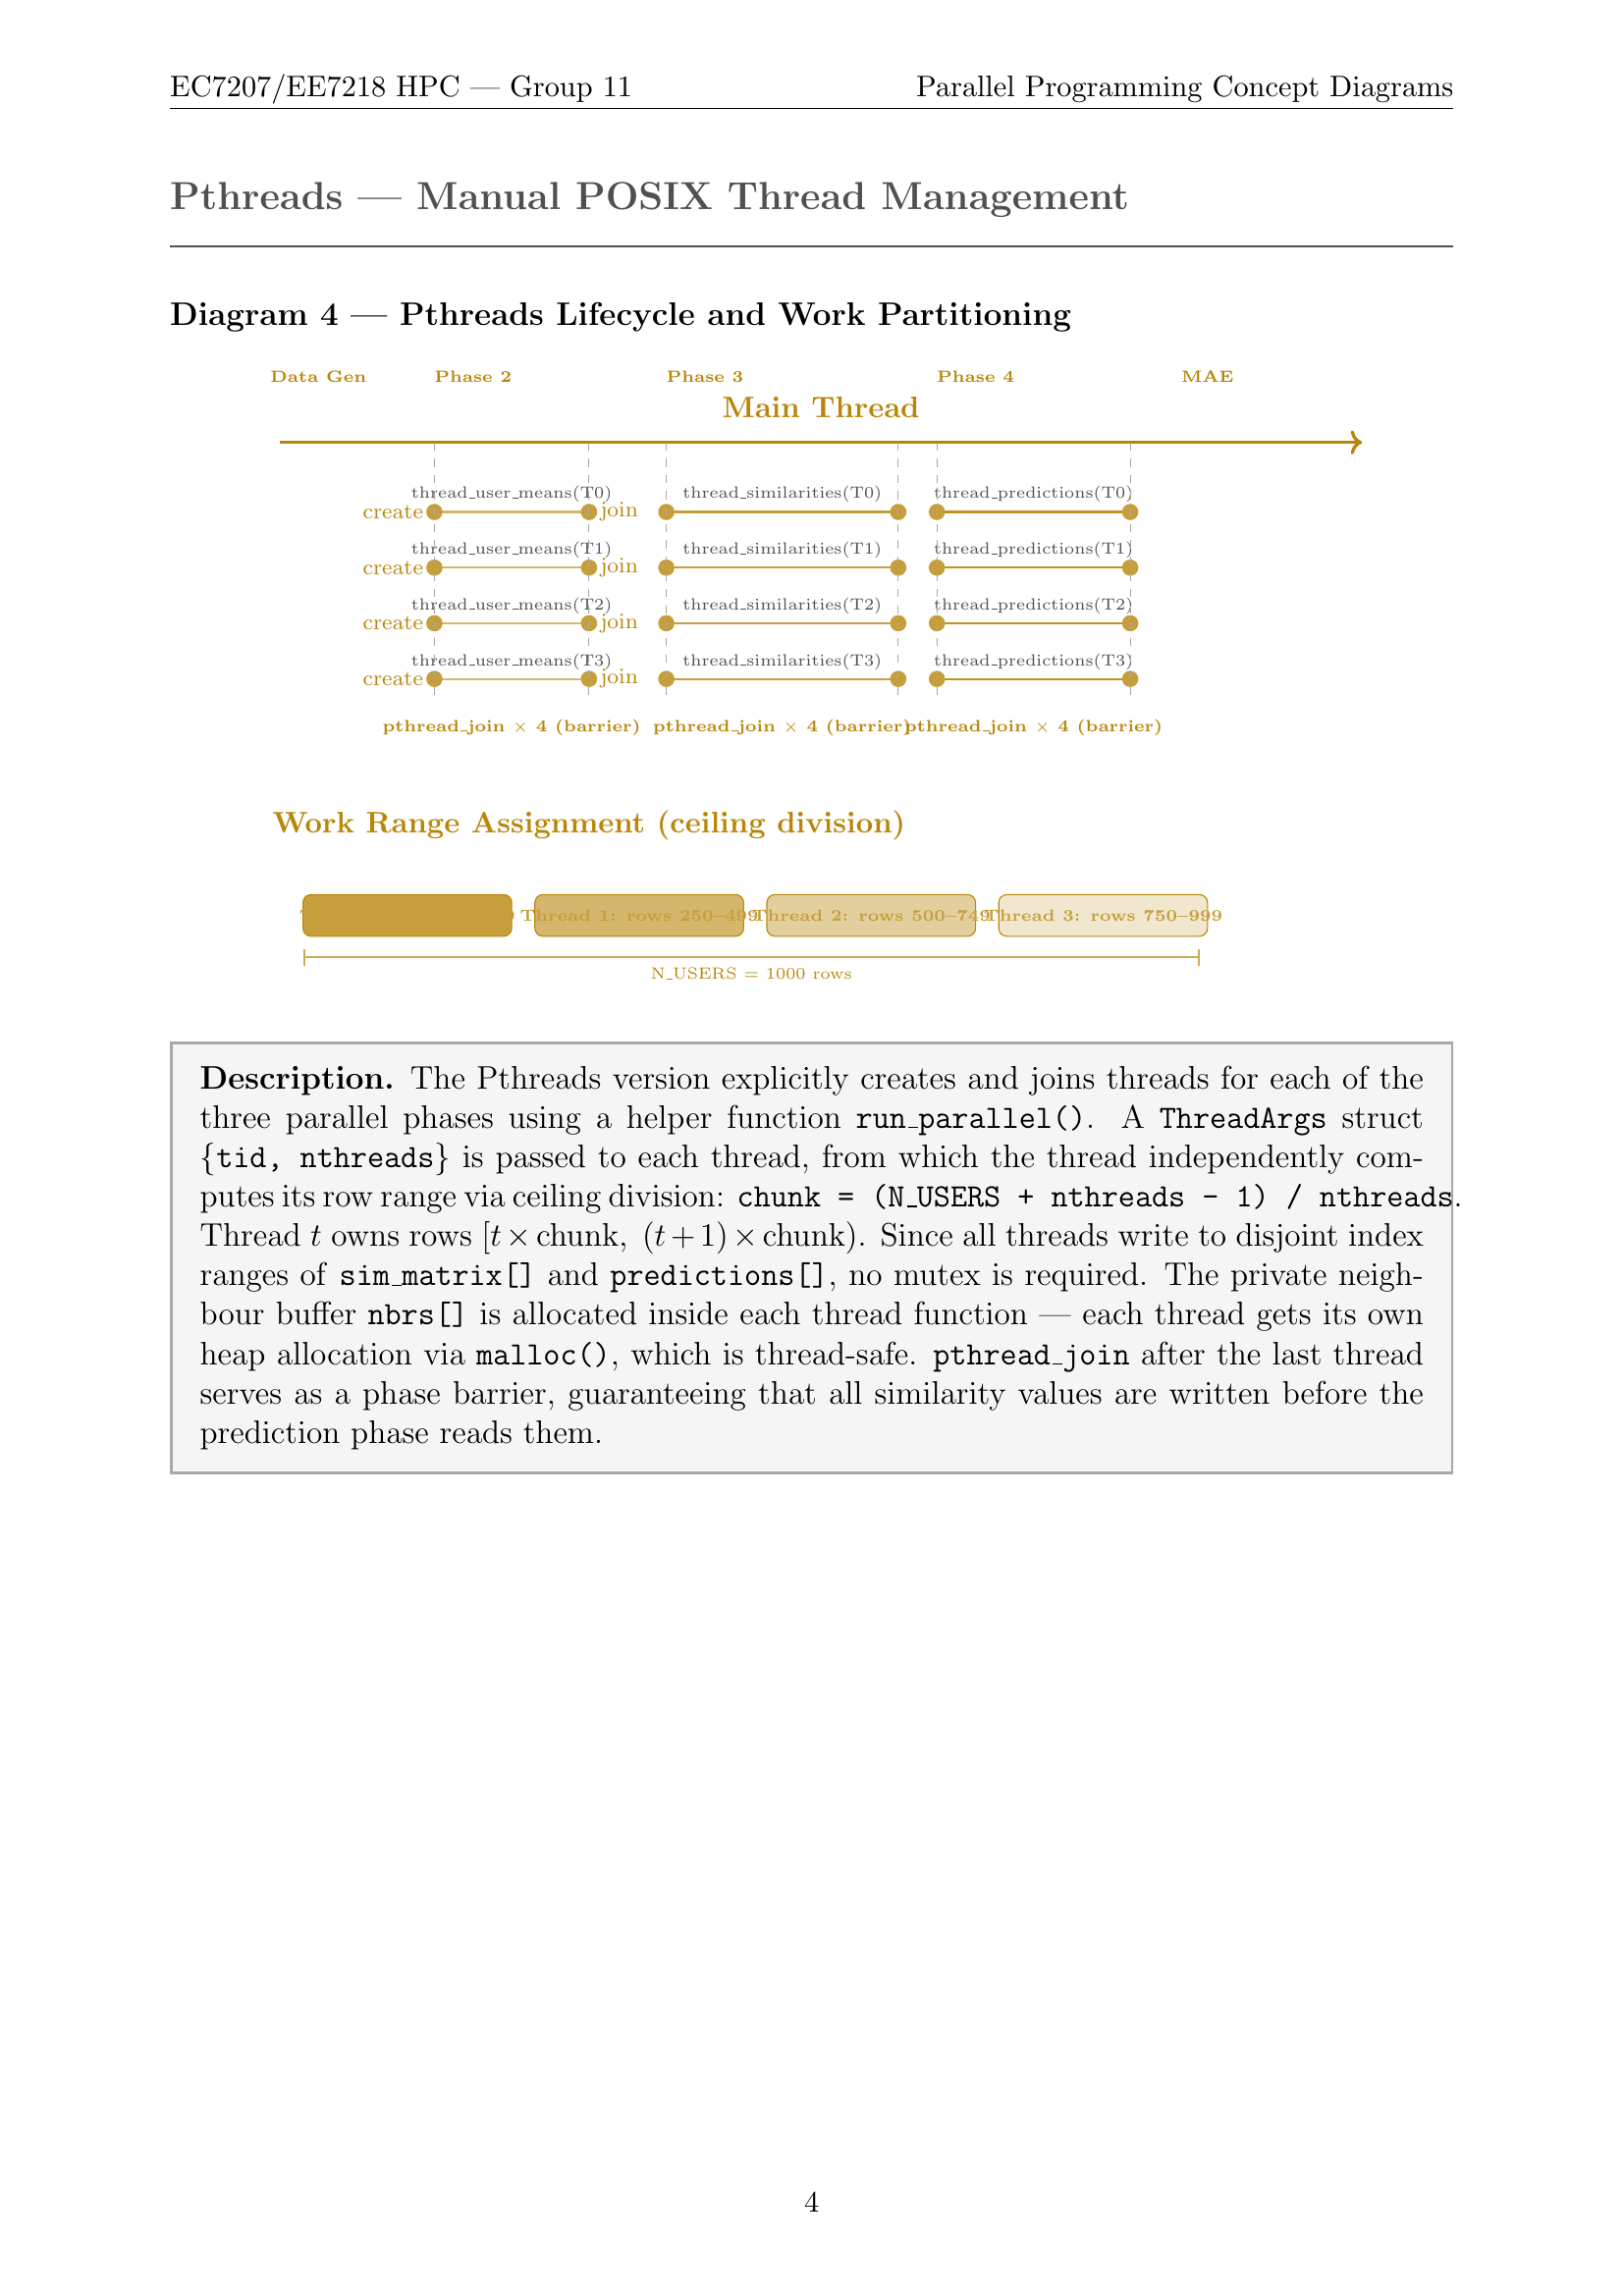
\includegraphics[width=0.85\textwidth]{../analysis_diagrams/charts/concept_pthreads.png}
  \caption{Manual POSIX-thread management. The \code{run\_parallel} harness
  creates $T$ threads with static \code{ceil}-division row ranges and joins them
  as a phase barrier, once per phase.}
\end{figure}

% ─────────────────────────────────────────────────────────────────────────────
\subsection{MPI --- Distributed-Memory Parallelism}

Each MPI rank is an independent process with its own private address space.
The $N=1{,}000$ users are divided evenly: rank $r$ owns rows
$[r \cdot N/P,\; (r{+}1)\cdot N/P)$.

\begin{table}[H]
\centering
\begin{tabular}{L{2cm} L{7cm} L{4cm}}
\toprule
\textbf{Phase} & \textbf{Strategy} & \textbf{Primitive} \\
\midrule
Phase 1 & All ranks call \code{srand(42)} --- no communication & --- \\
Phase 2 & Each rank computes its \code{user\_mean[]} slice      & \code{MPI\_Allgatherv} \\
Phase 3 & Each rank fills its rows of the sim matrix           & \code{MPI\_Allgatherv} \\
Phase 4 & Each rank predicts its own users                     & --- \\
Phase 5 & Local error sums to rank 0                           & \code{MPI\_Reduce(SUM)} \\
\bottomrule
\end{tabular}
\caption{MPI communication strategy per phase.}
\end{table}

The \code{MPI\_Allgatherv} for the $N \times N$ similarity matrix transfers
$\approx 4$\,MB at $N=1{,}000$.  This overhead limits single-node efficiency
but is the necessary mechanism for multi-node deployments.

\begin{figure}[H]
  \centering
  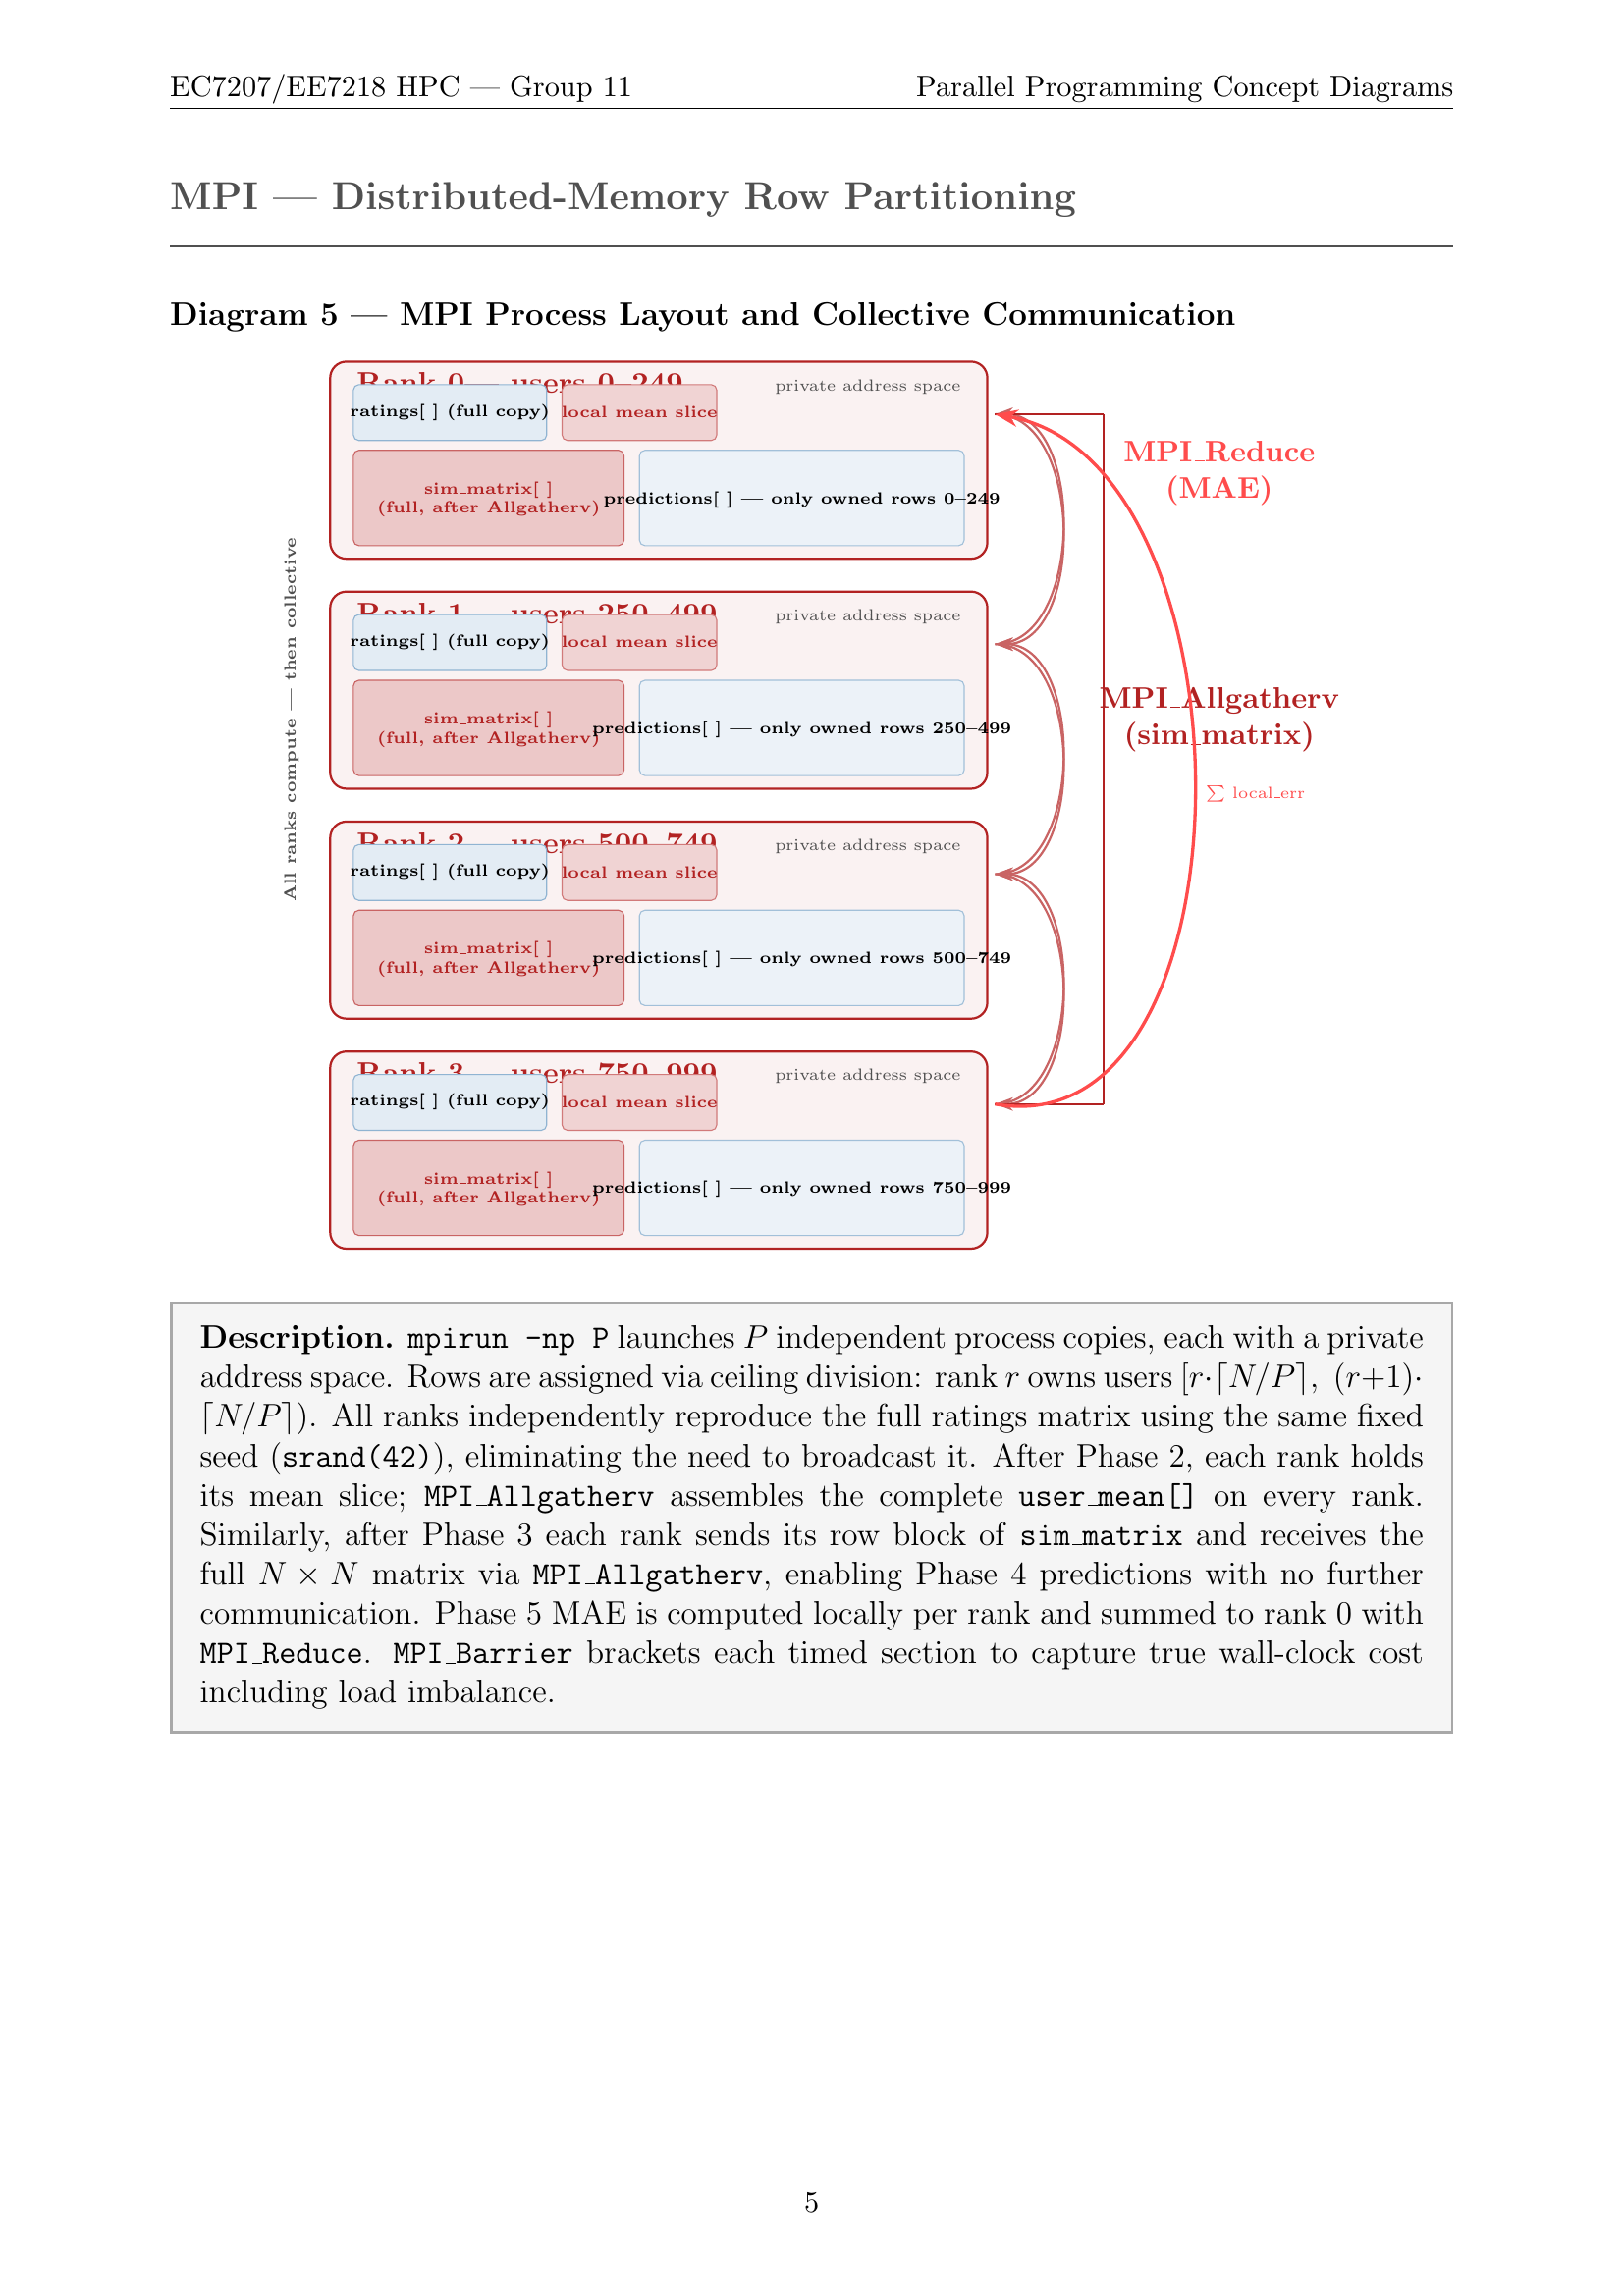
\includegraphics[width=0.85\textwidth]{../analysis_diagrams/charts/concept_mpi.png}
  \caption{MPI distributed-memory layout. Each rank is a separate process with
  a private address space; rows are assigned by \code{ceil}-division and the
  global similarity matrix is assembled with \code{MPI\_Allgatherv}, while
  MAE/RMSE use \code{MPI\_Reduce}.}
\end{figure}

% ─────────────────────────────────────────────────────────────────────────────
\subsection{CUDA --- GPU Massively Parallel Computing}

\textit{Note: CUDA code (\texttt{cuda/cuda\_recommender.cu}) is fully
implemented and benchmarked on an NVIDIA GeForce RTX 3050 Laptop GPU
(Ampere, compute capability 8.6, 16 SMs); measured results are reported in
Section~\ref{sec:cuda-results}.}

\begin{table}[H]
\centering
\begin{tabular}{L{4.5cm} L{5.5cm} L{4cm}}
\toprule
\textbf{Kernel} & \textbf{Launch config} & \textbf{Assignment} \\
\midrule
\code{kernel\_user\_means}  & \code{<<<(N+255)/256, 256>>>}           & 1 thread = 1 user \\
\code{kernel\_similarity}   & \code{dim3($\lceil N/16\rceil$, $\lceil N/16\rceil$), dim3(16,16)} & 1 thread = 1 $(u,v)$ pair \\
\code{kernel\_predictions}  & 2D grid, users $\times$ items            & 1 thread = 1 $(u,i)$ pair \\
\bottomrule
\end{tabular}
\caption{CUDA kernel configuration for $N=1{,}000$.}
\end{table}

The similarity kernel launches $63 \times 63 \times 256 = 1{,}016{,}064$
threads simultaneously.  Timing uses \code{cudaEventRecord} to separate
kernel-only time from \code{cudaMemcpy} transfer overhead.

\begin{figure}[H]
  \centering
  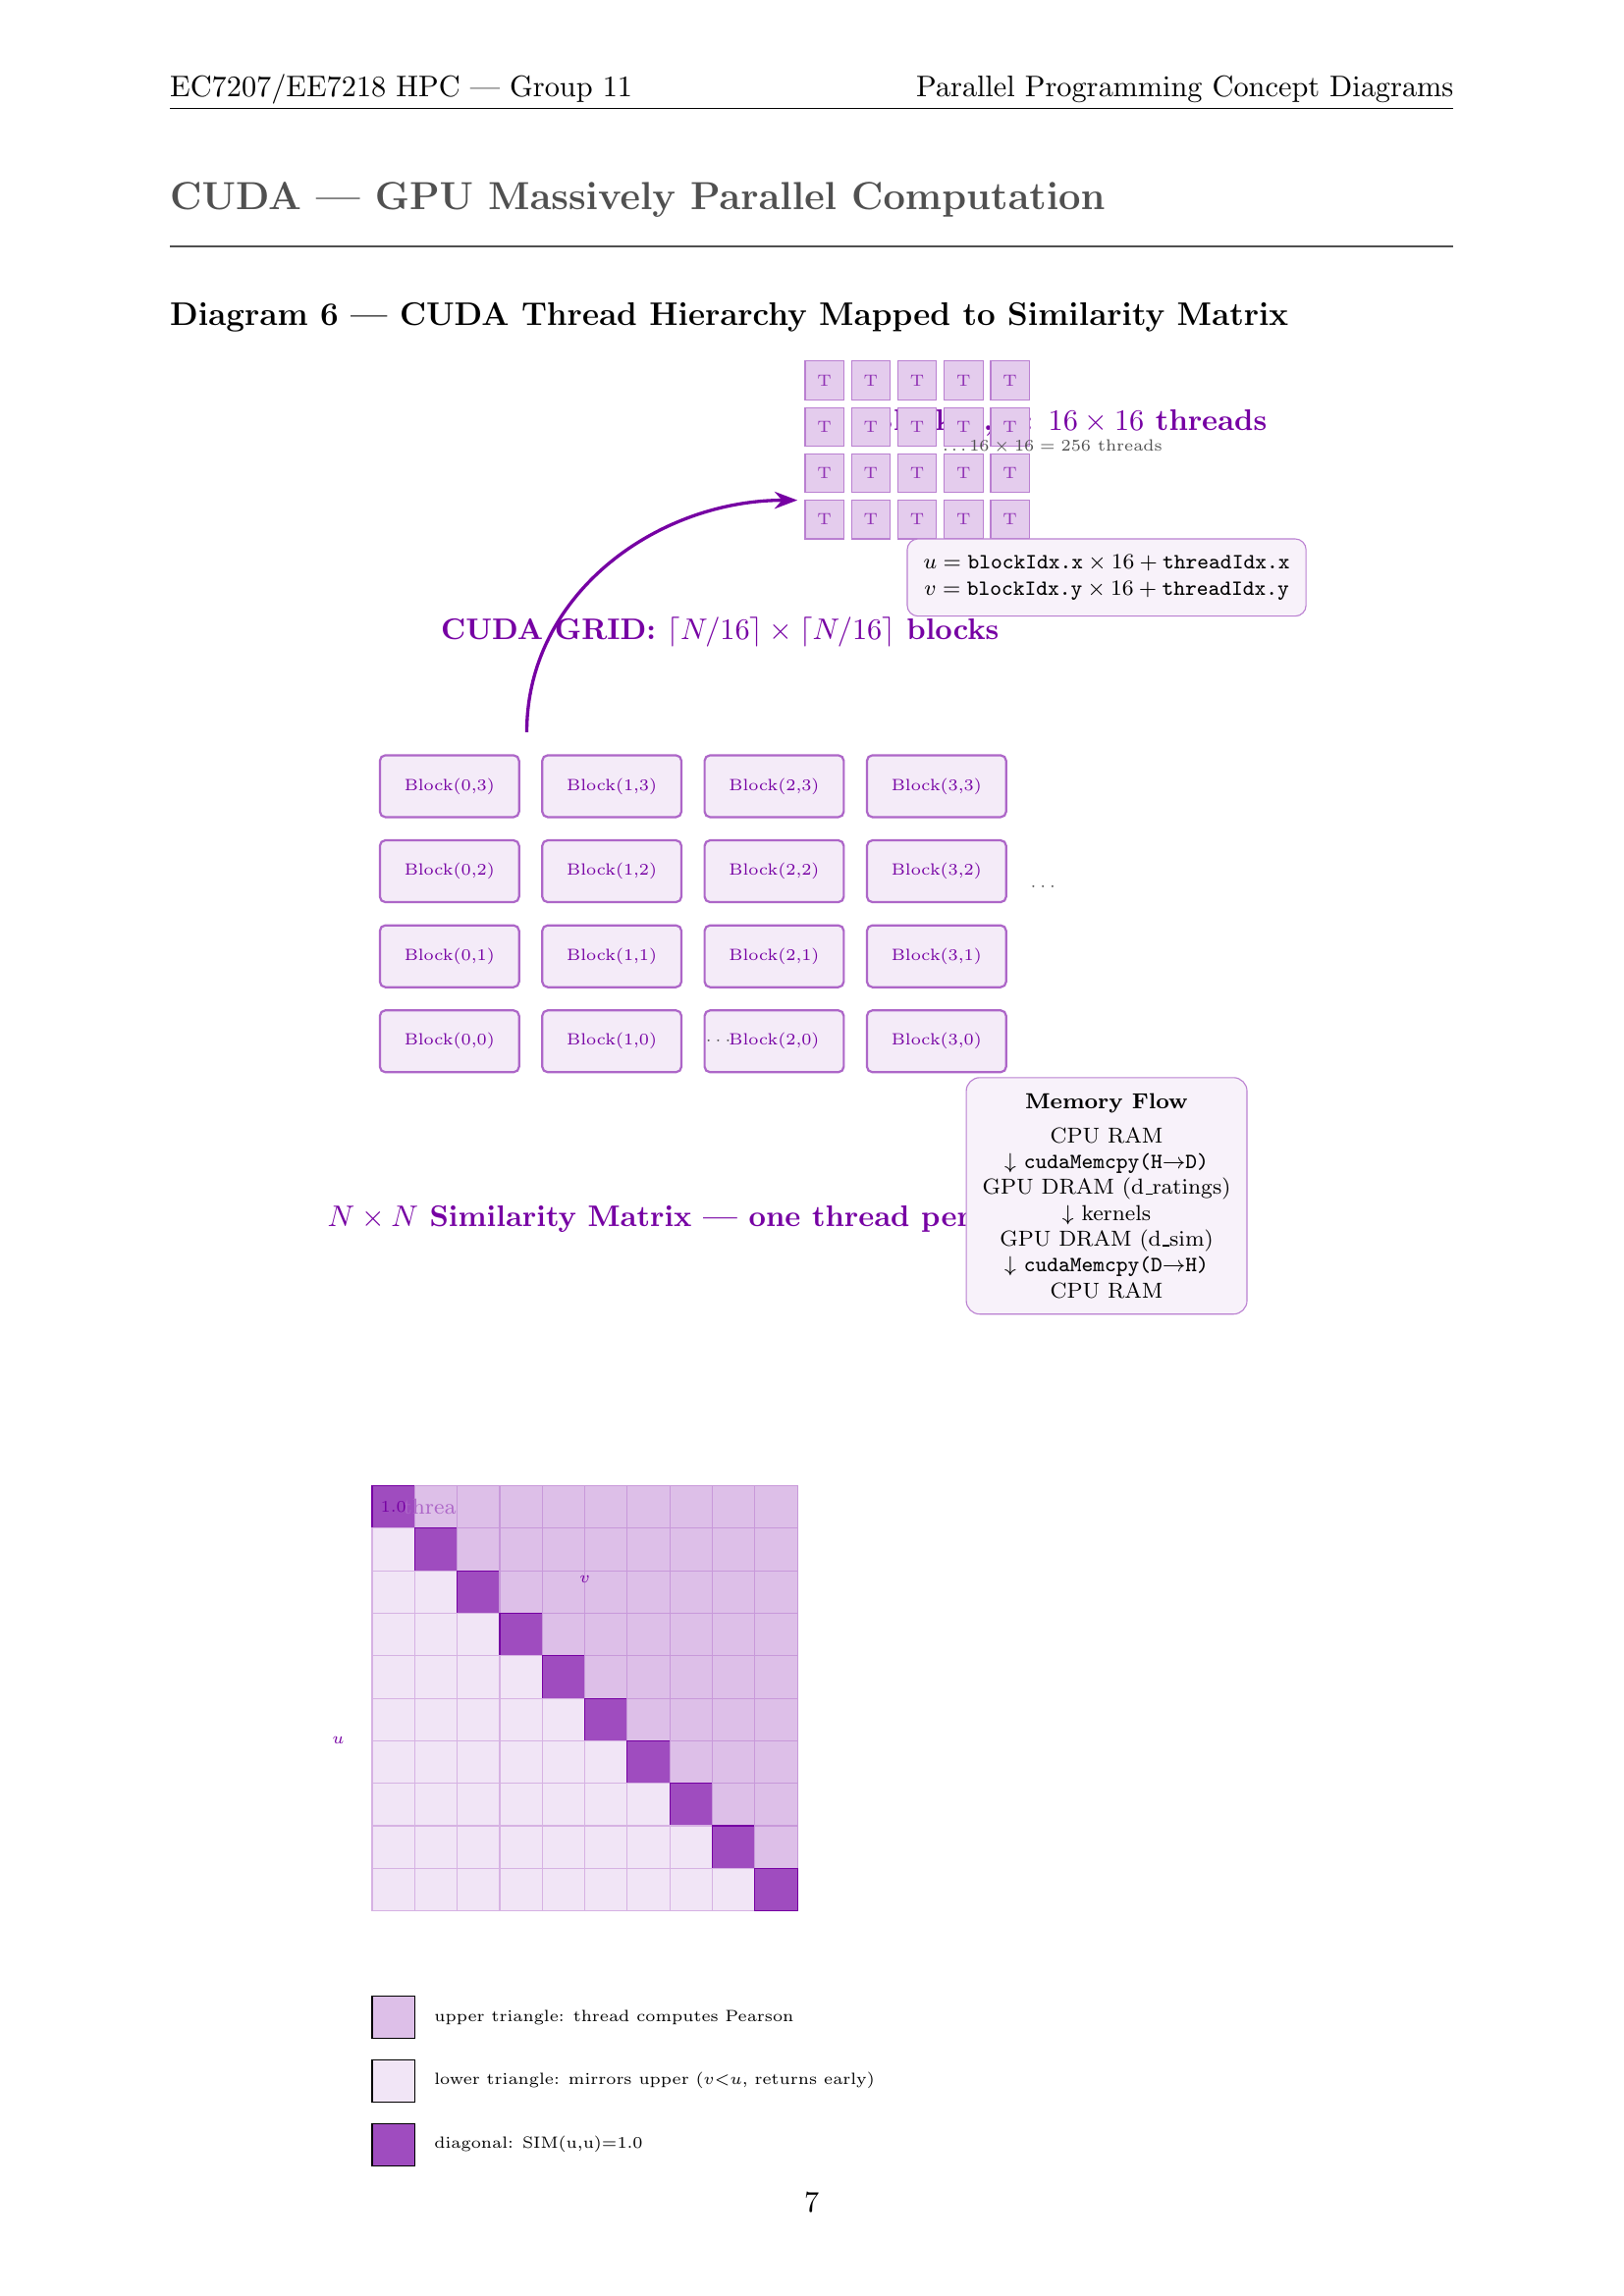
\includegraphics[width=0.85\textwidth]{../analysis_diagrams/charts/concept_cuda.png}
  \caption{CUDA GPU model. A 2D grid of thread blocks maps one thread to each
  $(u,v)$ similarity pair; the host transfers data, launches kernels, and copies
  results back. Benchmarked on an NVIDIA RTX 3050 (compute capability 8.6).}
\end{figure}

% ─────────────────────────────────────────────────────────────────────────────
\subsection{Hybrid MPI+OpenMP --- Two-Level Parallelism}

Combines MPI (coarse-grain inter-node) and OpenMP (fine-grain intra-node).
With $P$ MPI ranks and $T$ OpenMP threads per rank, the total worker count is
$P \times T$ while sending only $P$ messages per collective call.

\code{MPI\_Init\_thread(MPI\_THREAD\_FUNNELED)} ensures all MPI calls are made
exclusively from the main thread, after OpenMP parallel regions complete.

\begin{figure}[H]
  \centering
  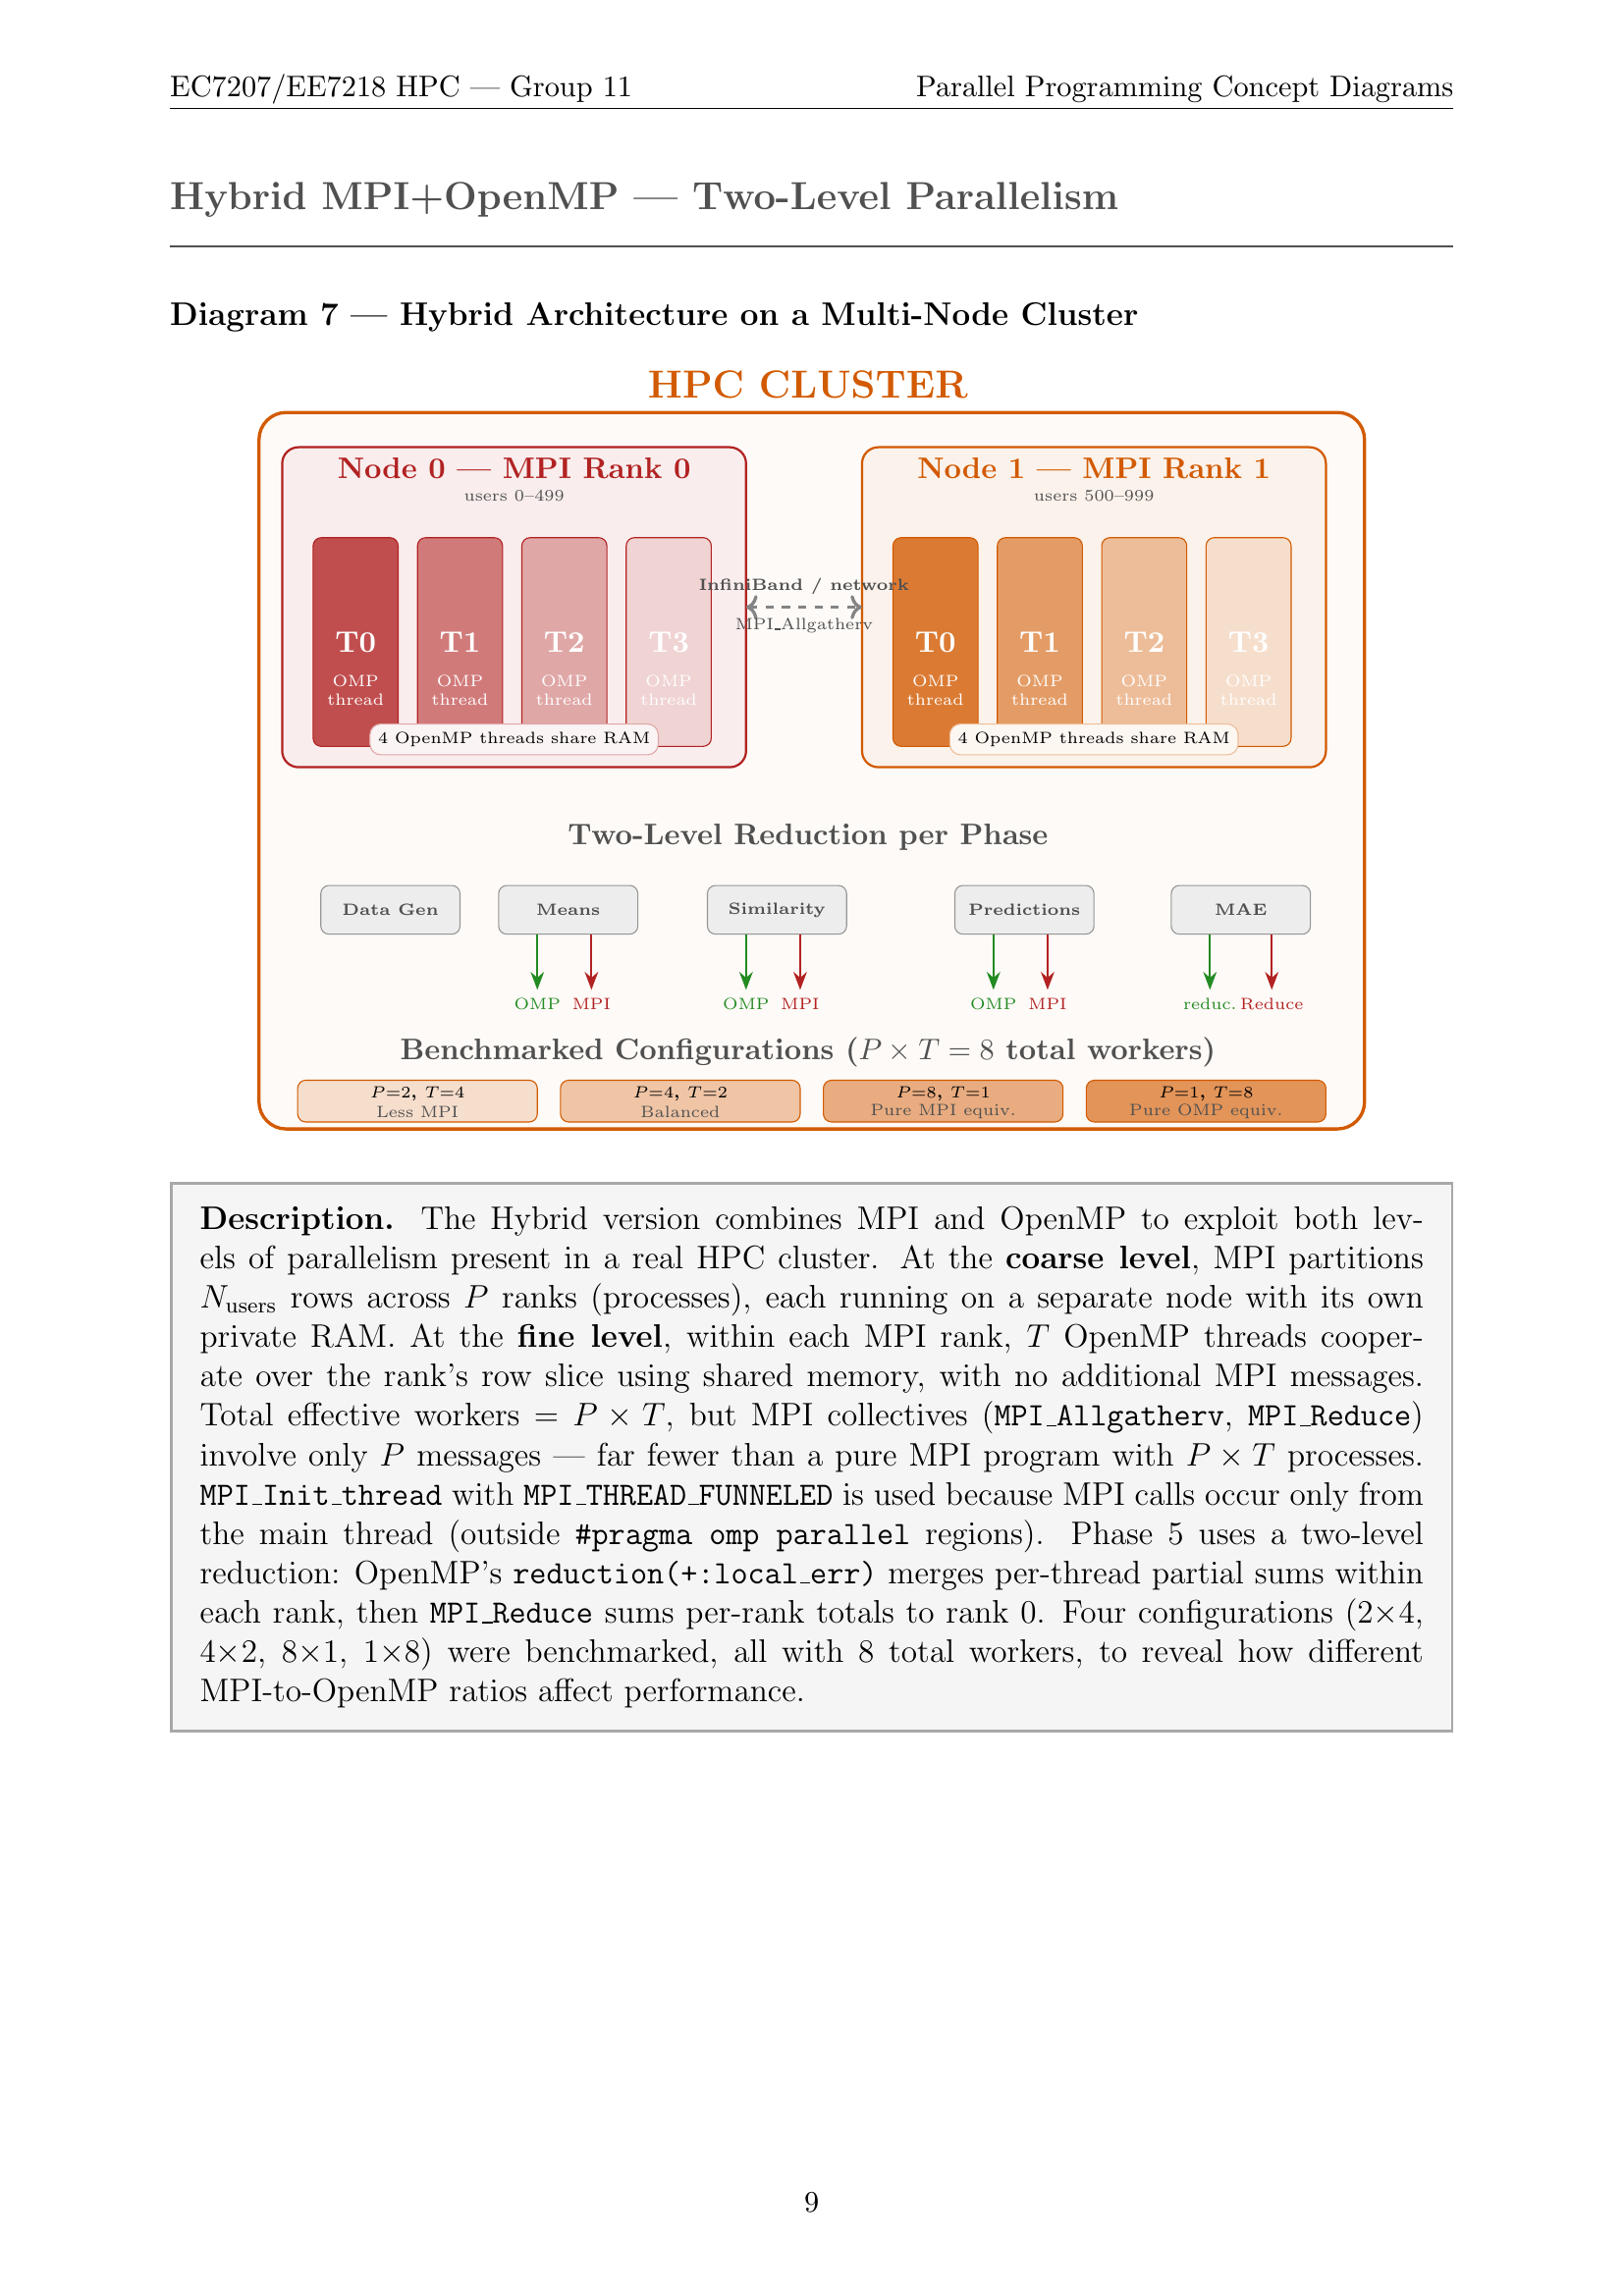
\includegraphics[width=0.85\textwidth]{../analysis_diagrams/charts/concept_hybrid.png}
  \caption{Hybrid two-level parallelism: MPI partitions user-rows across $P$
  ranks (coarse grain), and within each rank OpenMP spawns $T$ threads over that
  rank's rows (fine grain), for $P\times T$ total workers.}
\end{figure}

\begin{table}[H]
\centering
\begin{tabular}{C{2.5cm} C{2cm} C{2cm} L{7cm}}
\toprule
\textbf{Config} & \textbf{P} & \textbf{T} & \textbf{Characteristic} \\
\midrule
Hybrid 2$\times$4 & 2 & 4 & Fewer MPI messages; more shared-memory parallelism \\
Hybrid 4$\times$2 & 4 & 2 & Balanced communication vs.\ threading overhead \\
Hybrid 8$\times$1 & 8 & 1 & Equivalent to pure MPI \\
Hybrid 1$\times$8 & 1 & 8 & Pure OpenMP wrapped with MPI overhead \\
\bottomrule
\end{tabular}
\caption{Hybrid configurations (all 8 total workers).}
\end{table}

% ══════════════════════════════════════════════════════════════════════════════
\section{Accuracy Analysis --- Parallel vs.\ Serial}
% ══════════════════════════════════════════════════════════════════════════════

All parallel implementations are validated against the serial baseline using
two error metrics --- \textbf{Mean Absolute Error (MAE)} and \textbf{Root Mean
Square Error (RMSE)} --- together with a \textbf{similarity-matrix checksum}:
\[
  \text{MAE} = \frac{1}{|T|} \sum_{(u,i) \in T} |\hat{r}_{ui} - r_{ui}|,
  \qquad
  \text{RMSE} = \sqrt{\frac{1}{|T|} \sum_{(u,i) \in T} (\hat{r}_{ui} - r_{ui})^2}
  \qquad (|T| = 29{,}866)
\]

\textbf{MAE vs.\ RMSE.}  Both are reported, as suggested by the project
guideline.  MAE treats all errors equally on the bounded 1--5 rating scale,
while RMSE (always $\ge$ MAE) disproportionately penalises occasional large
errors --- here $\text{RMSE}=1.4579 > \text{MAE}=1.2574$ indicates a modest
spread of larger misses, expected for a 70\%-sparse synthetic matrix.

\begin{table}[H]
\centering
\begin{tabular}{L{2.6cm} C{1.4cm} C{1.5cm} C{1.5cm} C{2.6cm} R{2.6cm}}
\toprule
\textbf{Version} & \textbf{Workers} & \textbf{MAE} & \textbf{RMSE} &
\textbf{Matches Serial?} & \textbf{Sim Checksum} \\
\midrule
Serial         & 1   & 1.2574 & 1.4579 & baseline                & 942.387323 \\
OpenMP         & 1T  & 1.2574 & 1.4579 & YES $(\Delta=0.0000)$   & 942.387323 \\
OpenMP         & 2T  & 1.2574 & 1.4579 & YES $(\Delta=0.0000)$   & 942.387323 \\
OpenMP         & 4T  & 1.2574 & 1.4579 & YES $(\Delta=0.0000)$   & 942.387323 \\
OpenMP         & 8T  & 1.2574 & 1.4579 & YES $(\Delta=0.0000)$   & 942.387323 \\
Pthreads       & 1T  & 1.2574 & 1.4579 & YES $(\Delta=0.0000)$   & 942.387323 \\
Pthreads       & 2T  & 1.2574 & 1.4579 & YES $(\Delta=0.0000)$   & 942.387323 \\
Pthreads       & 4T  & 1.2574 & 1.4579 & YES $(\Delta=0.0000)$   & 942.387323 \\
Pthreads       & 8T  & 1.2574 & 1.4579 & YES $(\Delta=0.0000)$   & 942.387323 \\
MPI            & 1P  & 1.2574 & 1.4579 & YES $(\Delta=0.0000)$   & 942.387323 \\
MPI            & 2P  & 1.2574 & 1.4579 & YES $(\Delta=0.0000)$   & 942.387323 \\
MPI            & 4P  & 1.2574 & 1.4579 & YES $(\Delta=0.0000)$   & 942.387323 \\
MPI            & 8P  & 1.2574 & 1.4579 & YES $(\Delta=0.0000)$   & 942.387323 \\
Hybrid 2$\times$4 & 8 & 1.2574 & 1.4579 & YES $(\Delta=0.0000)$ & 942.387323 \\
Hybrid 4$\times$2 & 8 & 1.2574 & 1.4579 & YES $(\Delta=0.0000)$ & 942.387323 \\
Hybrid 8$\times$1 & 8 & 1.2574 & 1.4579 & YES $(\Delta=0.0000)$ & 942.387323 \\
Hybrid 1$\times$8 & 8 & 1.2574 & 1.4579 & YES $(\Delta=0.0000)$ & 942.387323 \\
CUDA           & GPU & 1.2574 & 1.4579 & YES $(\Delta=0.0000)$   & 942.387323 \\
\bottomrule
\end{tabular}
\caption{Accuracy correctness. All 18 runs (17 CPU + 1 GPU) produce identical
MAE, RMSE, and similarity checksum.}
\end{table}

All 18 runs produce MAE = \textbf{1.2574}, RMSE = \textbf{1.4579}, and
checksum = \textbf{942.387323} --- confirming zero race conditions and correct
partitioning across every implementation.  Crucially, the CUDA version, despite
using completely different floating-point hardware and a register-based top-$K$
selection (vs.\ the CPU's \code{qsort}), reproduces the serial result exactly to
four decimal places, validating the GPU kernels.

\begin{figure}[H]
  \centering
  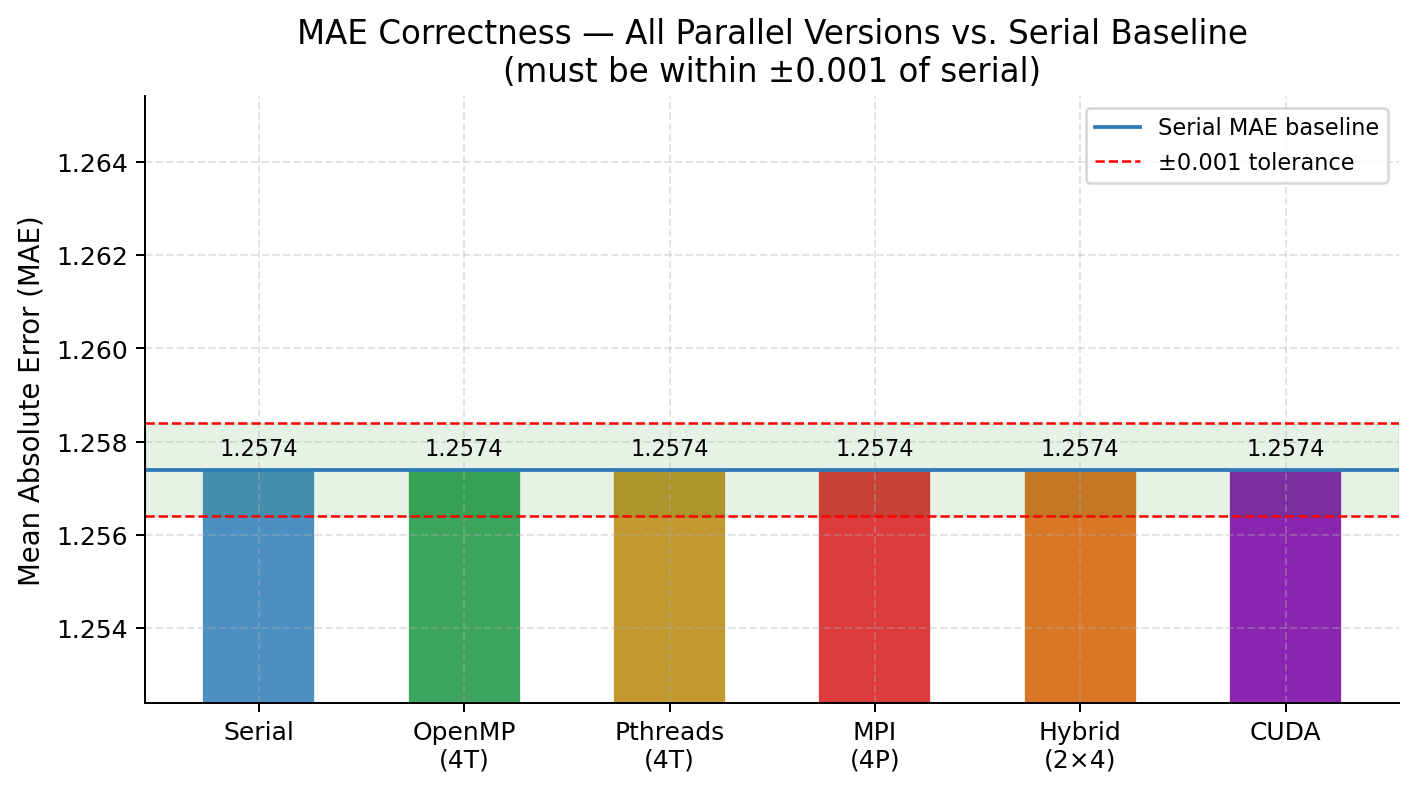
\includegraphics[width=0.80\textwidth]{../analysis_diagrams/charts/mae_comparison.png}
  \caption{MAE correctness. All bars lie within the $\pm0.001$ tolerance band.}
\end{figure}

% ══════════════════════════════════════════════════════════════════════════════
\section{Timing Measurements and Performance Analysis}
% ══════════════════════════════════════════════════════════════════════════════

\subsection{Performance Metric Definitions}

\[
  S(p) = \frac{T_{\text{serial}}}{T_{\text{parallel}}(p)}
  \qquad
  E(p) = \frac{S(p)}{p}
  \qquad
  S_{\max}(p) = \frac{1}{f + (1-f)/p}
  \quad (f \approx 0.04)
\]

At $p=8$: $S_{\max}(8) = 1/(0.04+0.96/8) \approx 6.25\times$.

\subsection{Serial Baseline}

\begin{table}[H]
\centering
\begin{tabular}{lrr}
\toprule
\textbf{Phase} & \textbf{Time (s)} & \textbf{\% of Total} \\
\midrule
Similarity matrix (Phase 3) & 1.3549 & 16.2\% \\
Prediction phase (Phase 4)  & 7.0277 & 83.8\% \\
\textbf{Total (sim + pred)} & \textbf{8.3826} & \textbf{100\%} \\
\bottomrule
\end{tabular}
\caption{Serial baseline timing ($N=M=1{,}000$).}
\end{table}

\subsection{OpenMP --- Varying Thread Count}

\begin{table}[H]
\centering
\begin{tabular}{C{2.5cm} R{2.5cm} R{2.5cm} R{2.5cm} R{2.5cm} R{2.5cm}}
\toprule
\textbf{Threads} & \textbf{Sim (s)} & \textbf{Pred (s)} &
\textbf{Total (s)} & \textbf{Speedup} & \textbf{Efficiency} \\
\midrule
1 & 1.6102 & 7.2447 & 8.8549 & 0.95 & 0.95 \\
2 & 0.8114 & 3.6679 & 4.4792 & 1.87 & 0.94 \\
4 & 0.4457 & 2.0704 & 2.5161 & 3.33 & 0.83 \\
\textbf{8} & \textbf{0.2369} & \textbf{1.0903} & \textbf{1.3272} & \textbf{6.32} & \textbf{0.79} \\
\bottomrule
\end{tabular}
\caption{OpenMP results. Speedup relative to serial baseline (8.3826 s).}
\end{table}

\subsection{Pthreads --- Varying Thread Count}

\begin{table}[H]
\centering
\begin{tabular}{C{2.5cm} R{2.5cm} R{2.5cm} R{2.5cm} R{2.5cm} R{2.5cm}}
\toprule
\textbf{Threads} & \textbf{Sim (s)} & \textbf{Pred (s)} &
\textbf{Total (s)} & \textbf{Speedup} & \textbf{Efficiency} \\
\midrule
1 & 1.3333 & 7.3272 & 8.6605 & 0.97 & 0.97 \\
2 & 0.9816 & 3.7720 & 4.7536 & 1.76 & 0.88 \\
4 & 0.5999 & 2.0688 & 2.6687 & 3.14 & 0.79 \\
\textbf{8} & \textbf{0.3519} & \textbf{1.1275} & \textbf{1.4794} & \textbf{5.67} & \textbf{0.71} \\
\bottomrule
\end{tabular}
\caption{Pthreads results.}
\end{table}

\subsection{MPI --- Varying Process Count}

\begin{table}[H]
\centering
\begin{tabular}{C{2.5cm} R{2.5cm} R{2.5cm} R{2.5cm} R{2.5cm} R{2.5cm}}
\toprule
\textbf{Processes} & \textbf{Sim (s)} & \textbf{Pred (s)} &
\textbf{Total (s)} & \textbf{Speedup} & \textbf{Efficiency} \\
\midrule
1 & 3.1994 & 7.4317 & 10.6311 & 0.79 & 0.79 \\
2 & 1.6090 & 3.8648 & 5.4739 & 1.53 & 0.77 \\
4 & 0.9031 & 2.1281 & 3.0311 & 2.77 & 0.69 \\
\textbf{8} & \textbf{0.4846} & \textbf{1.1550} & \textbf{1.6395} & \textbf{5.11} & \textbf{0.64} \\
\bottomrule
\end{tabular}
\caption{MPI results. MPI 1P (10.63 s) $>$ serial (8.38 s) due to process startup
and \code{MPI\_Allgatherv} overhead at $P=1$ --- expected, not a bug.}
\end{table}

\subsection{Hybrid MPI+OpenMP --- Fixed 8 Total Workers}

\begin{table}[H]
\centering
\begin{tabular}{L{3cm} C{1.5cm} C{1.5cm} R{2cm} R{2cm} R{2cm} R{1.8cm} R{2cm}}
\toprule
\textbf{Config} & \textbf{P} & \textbf{T} &
\textbf{Sim (s)} & \textbf{Pred (s)} & \textbf{Total (s)} &
\textbf{S} & \textbf{E} \\
\midrule
Hybrid 2$\times$4 & 2 & 4 & 1.2032 & 2.7766 & 3.9798 & 2.11 & 0.26 \\
Hybrid 4$\times$2 & 4 & 2 & 0.6169 & 1.1631 & 1.7800 & 4.71 & 0.59 \\
\textbf{Hybrid 8$\times$1} & \textbf{8} & \textbf{1} & \textbf{0.5149} & \textbf{1.1904} & \textbf{1.7053} & \textbf{4.92} & \textbf{0.61} \\
Hybrid 1$\times$8 & 1 & 8 & 2.4520 & 5.4913 & 7.9433 & 1.06 & 0.13 \\
\bottomrule
\end{tabular}
\caption{Hybrid results (8 total workers). Best config is Hybrid 8$\times$1 --- essentially pure MPI.}
\end{table}

\subsection{CUDA --- GPU Benchmark}
\label{sec:cuda-results}

The CUDA version was benchmarked on the same machine's
\textbf{NVIDIA GeForce RTX 3050 Laptop GPU} (Ampere, compute capability 8.6,
16 SMs, 4\,GB), compiled with \code{nvcc -O2 -arch=sm\_86}.  Speedup is reported
against the serial baseline ($T_{\text{serial}} = 8.3826$\,s).

\begin{table}[H]
\centering
\begin{tabular}{L{5cm} R{2.5cm} R{3cm}}
\toprule
\textbf{Phase / Metric} & \textbf{Time (s)} & \textbf{Notes} \\
\midrule
H$\rightarrow$D transfer (ratings) & 0.0009 & PCIe, one-off \\
Similarity matrix (Phase 3) & 0.0862 & GPU kernel (CUDA events) \\
Prediction phase (Phase 4)  & 0.1343 & GPU kernel (CUDA events) \\
\textbf{Total (sim + pred)}  & \textbf{0.2205} & kernel-only \\
\midrule
Speedup vs.\ serial          & \textbf{38.02$\times$} & vs.\ serial 8.3826\,s \\
\bottomrule
\end{tabular}
\caption{CUDA timing on the RTX 3050 ($N=M=1{,}000$). The similarity kernel
launches $63\times63\times256 = 1{,}016{,}064$ threads; kernel time is isolated
from host\,$\leftrightarrow$\,device transfers via \code{cudaEventRecord}.}
\end{table}

The GPU completes the combined similarity + prediction work in \textbf{0.22\,s}
--- roughly \textbf{38$\times$} faster than the serial baseline and about
\textbf{6$\times$} faster than the best 8-thread CPU configuration --- because
the embarrassingly parallel $(u,v)$ and $(u,i)$ workloads map directly onto the
GPU's thousands of cores.  Host\,$\leftrightarrow$\,device transfer cost is
negligible (sub-millisecond) since the ratings matrix stays resident on the
device across all three kernels.

\subsection{Performance Charts}

\begin{figure}[H]
  \centering
  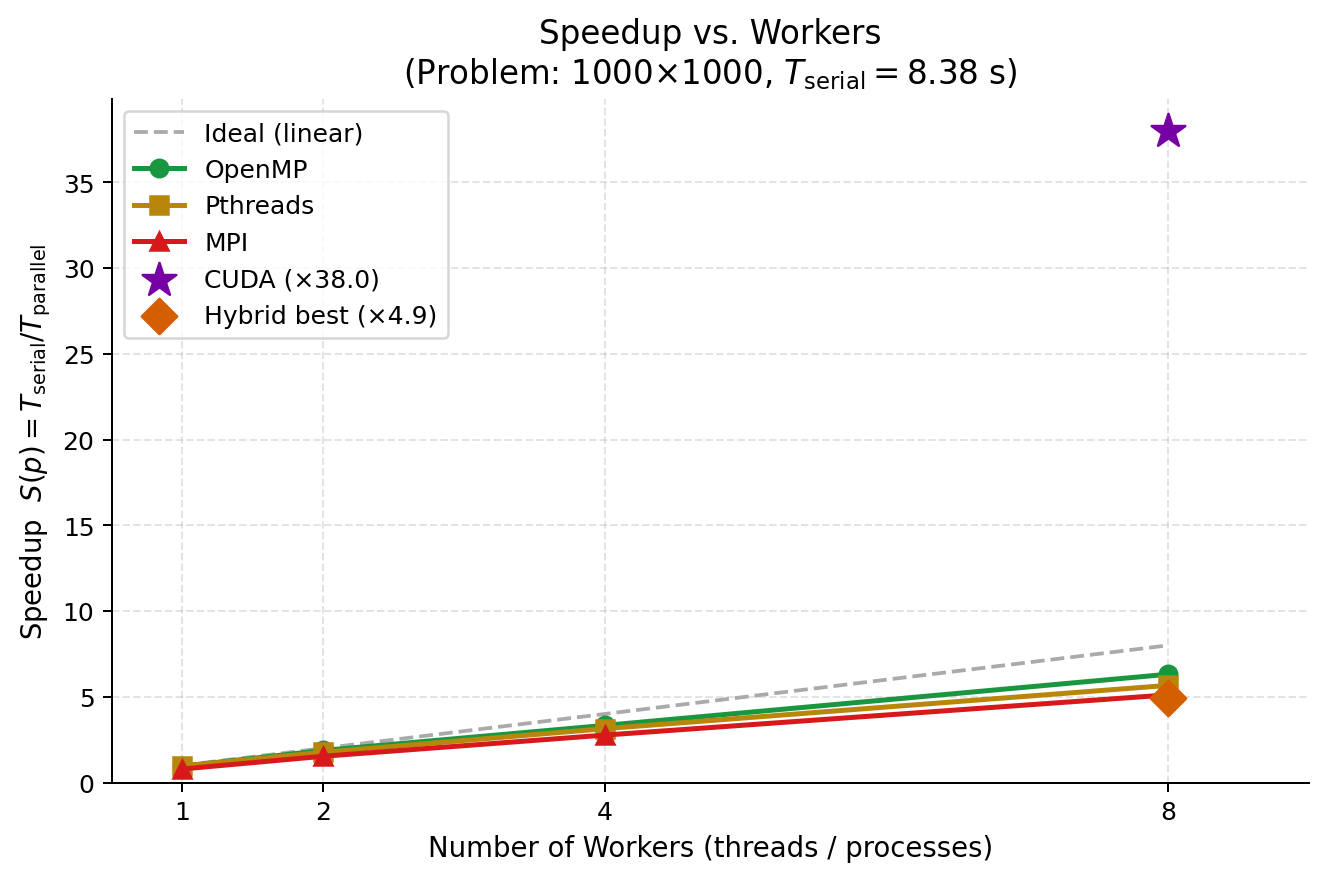
\includegraphics[width=\textwidth]{../analysis_diagrams/charts/speedup_comparison.png}
  \caption{Speedup vs.\ workers. Dashed = ideal linear. $\blacklozenge$ = best Hybrid (8$\times$1).}
\end{figure}

\begin{figure}[H]
  \centering
  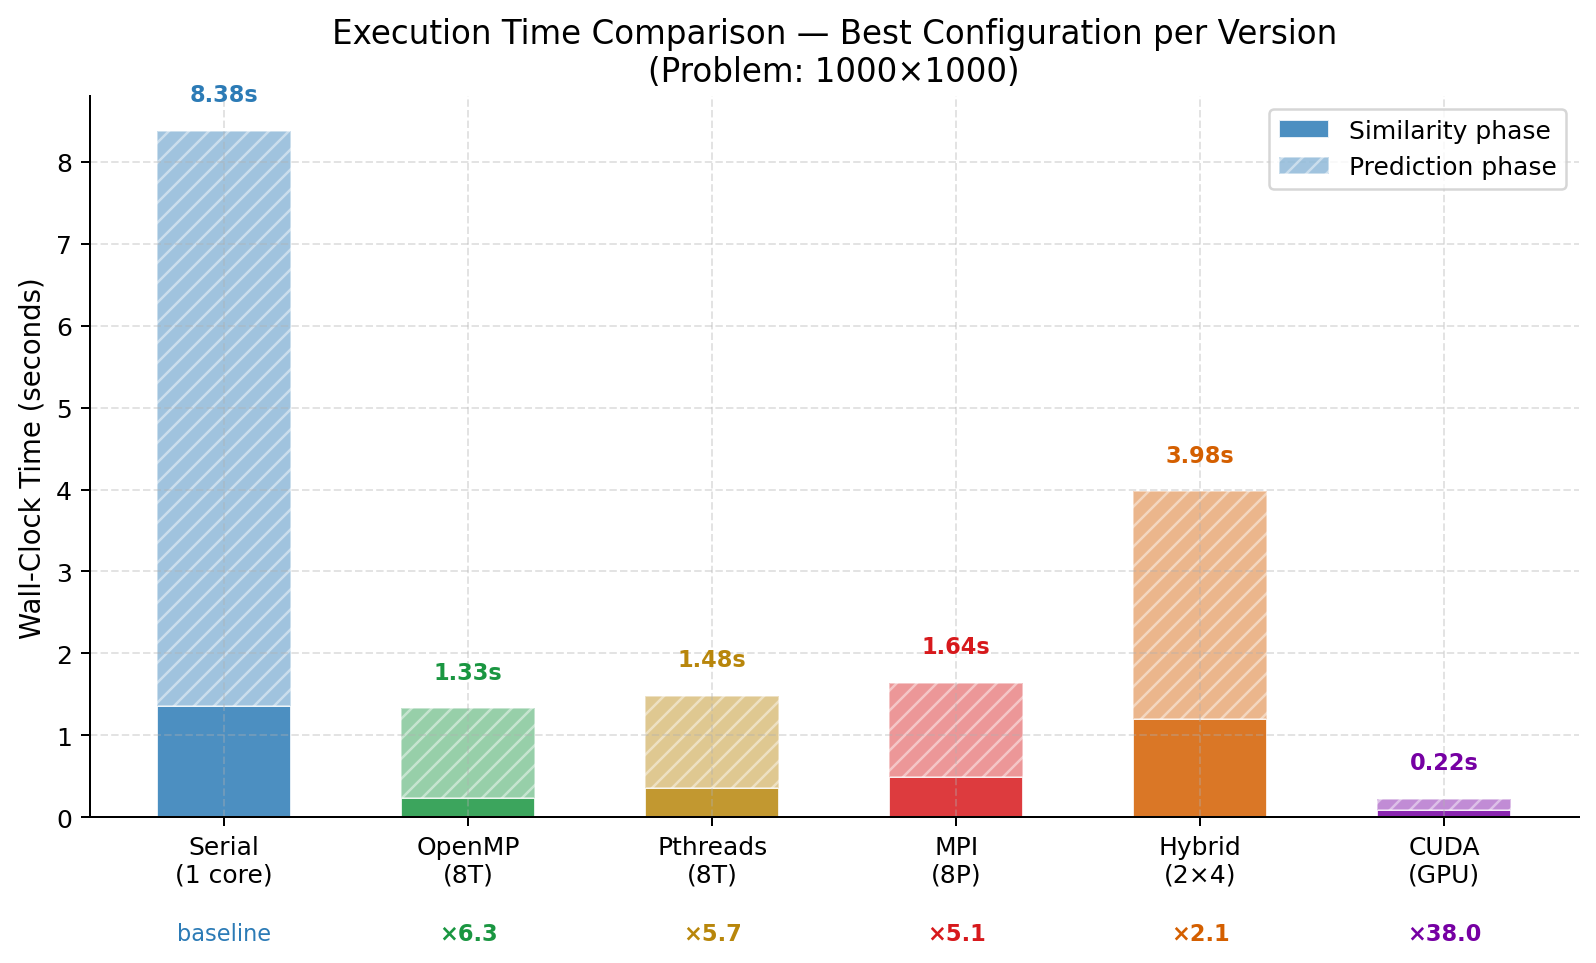
\includegraphics[width=\textwidth]{../analysis_diagrams/charts/execution_time_bar.png}
  \caption{Wall-clock time --- best config per version. Solid = similarity phase; hatched = prediction.}
\end{figure}

\begin{figure}[H]
  \centering
  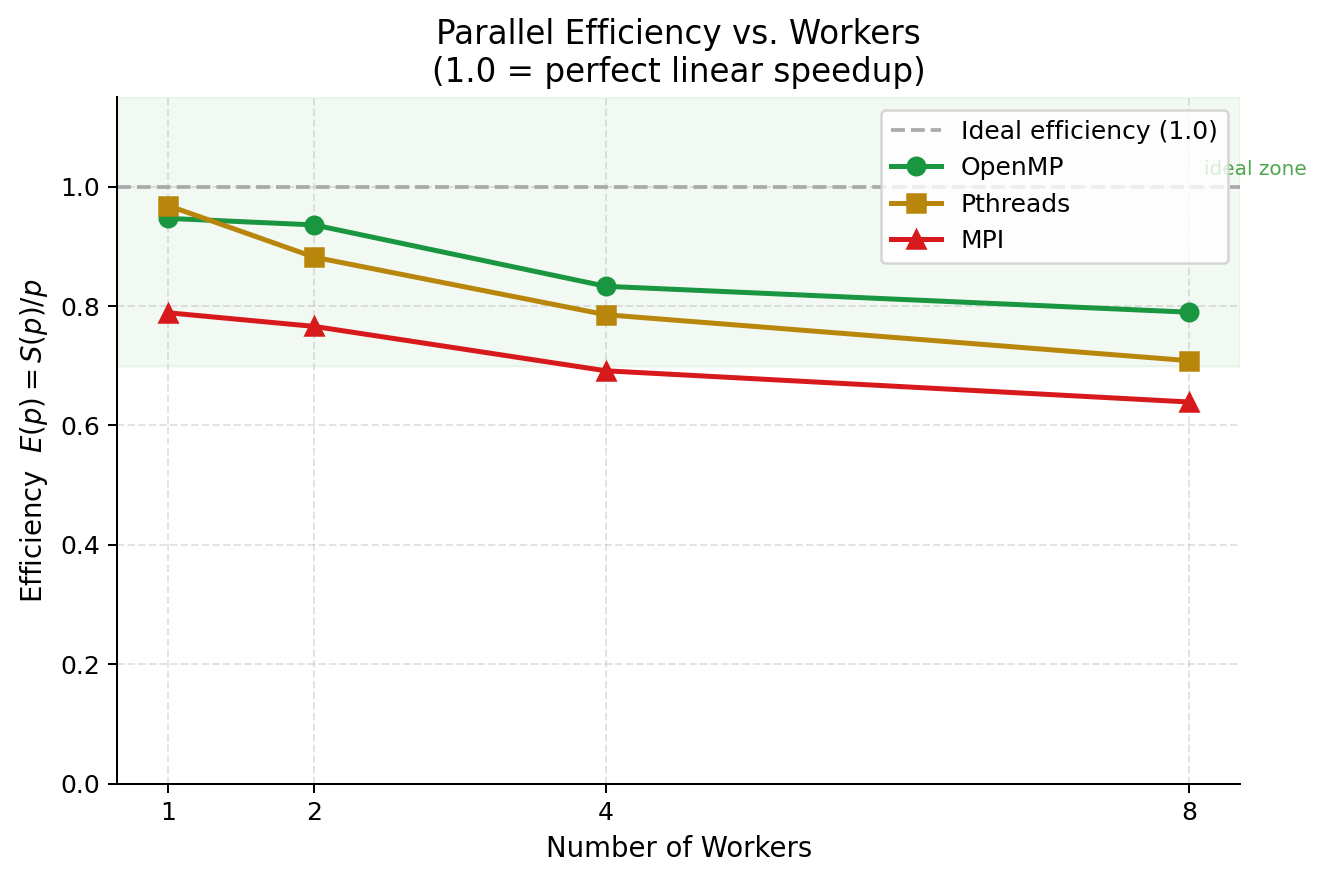
\includegraphics[width=\textwidth]{../analysis_diagrams/charts/efficiency_plot.png}
  \caption{Parallel efficiency $E(p)=S(p)/p$. Green zone ($>0.70$) = good utilisation.}
\end{figure}

\begin{figure}[H]
  \centering
  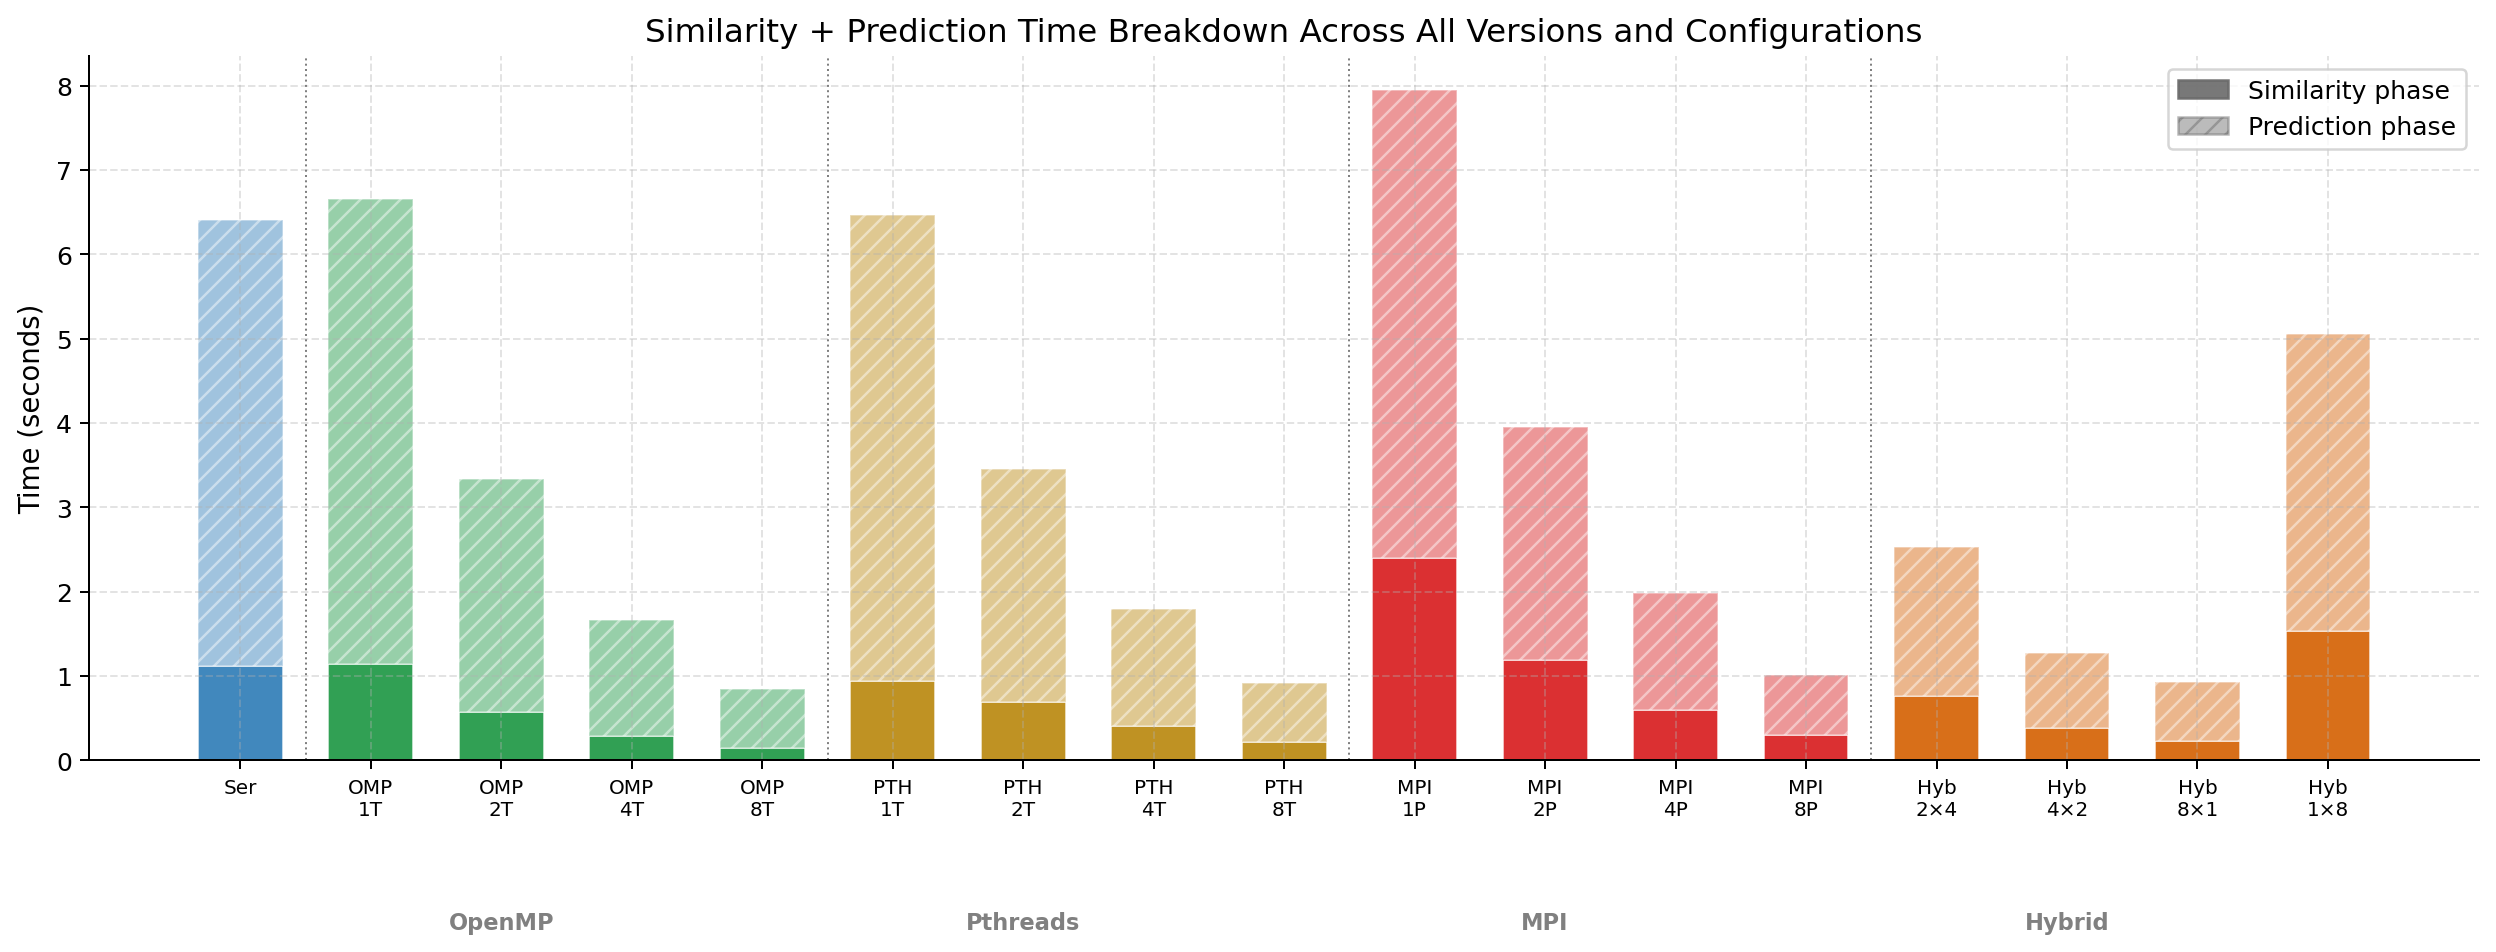
\includegraphics[width=\textwidth]{../analysis_diagrams/charts/sim_pred_breakdown.png}
  \caption{Similarity + Prediction time breakdown across all versions and configurations.}
\end{figure}

\begin{figure}[H]
  \centering
  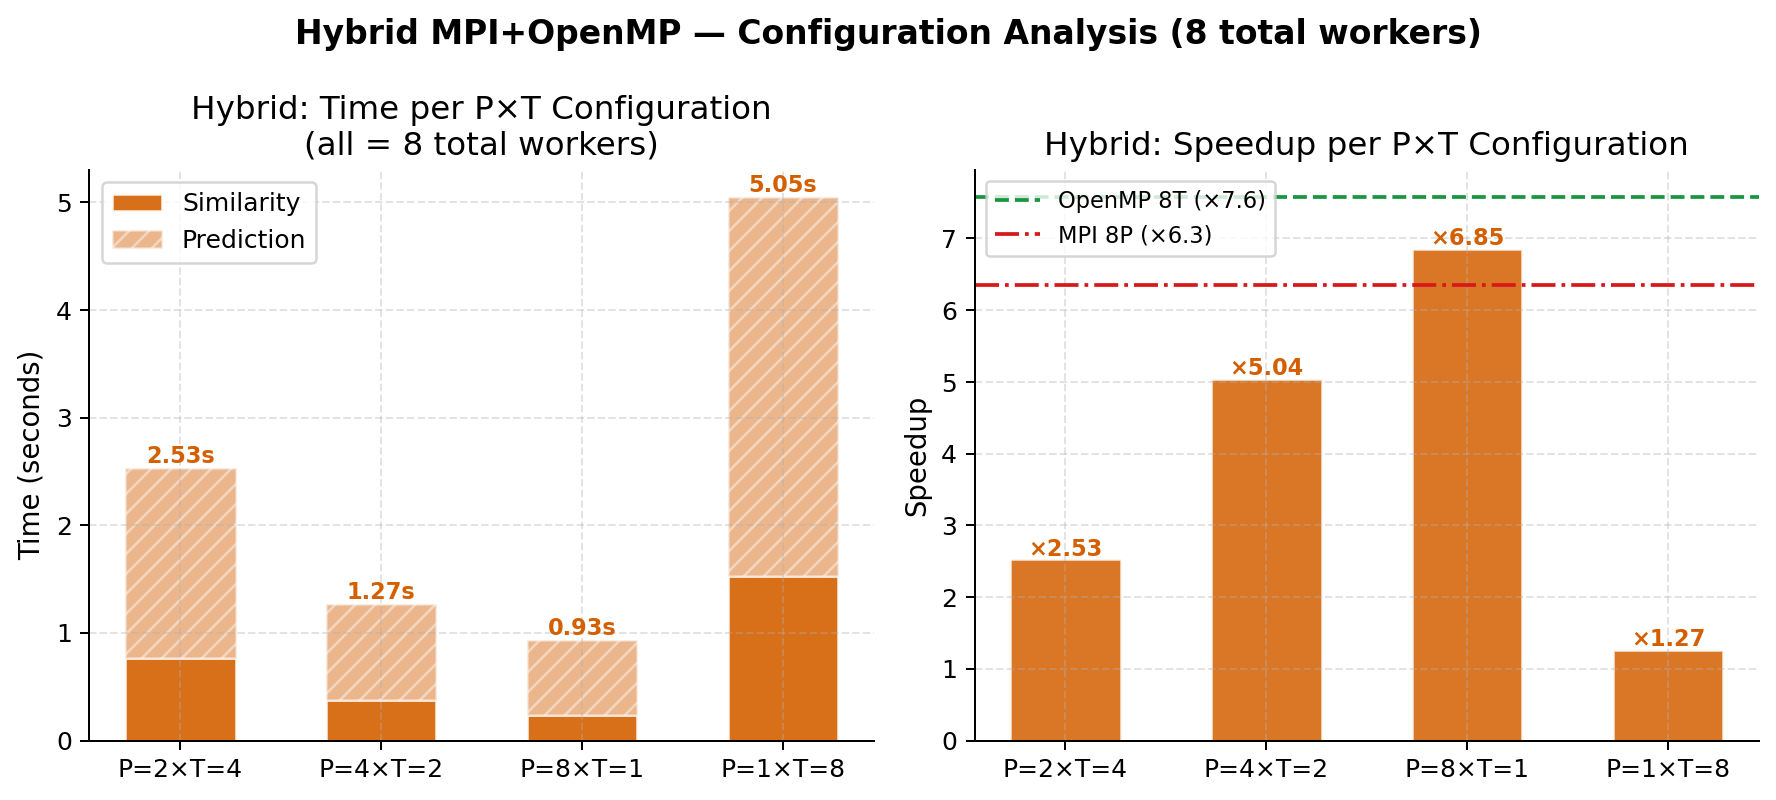
\includegraphics[width=\textwidth]{../analysis_diagrams/charts/hybrid_configs.png}
  \caption{Hybrid MPI+OpenMP configuration analysis. Left: time. Right: speedup vs.\ OpenMP-8T and MPI-8P.}
\end{figure}

\begin{figure}[H]
  \centering
  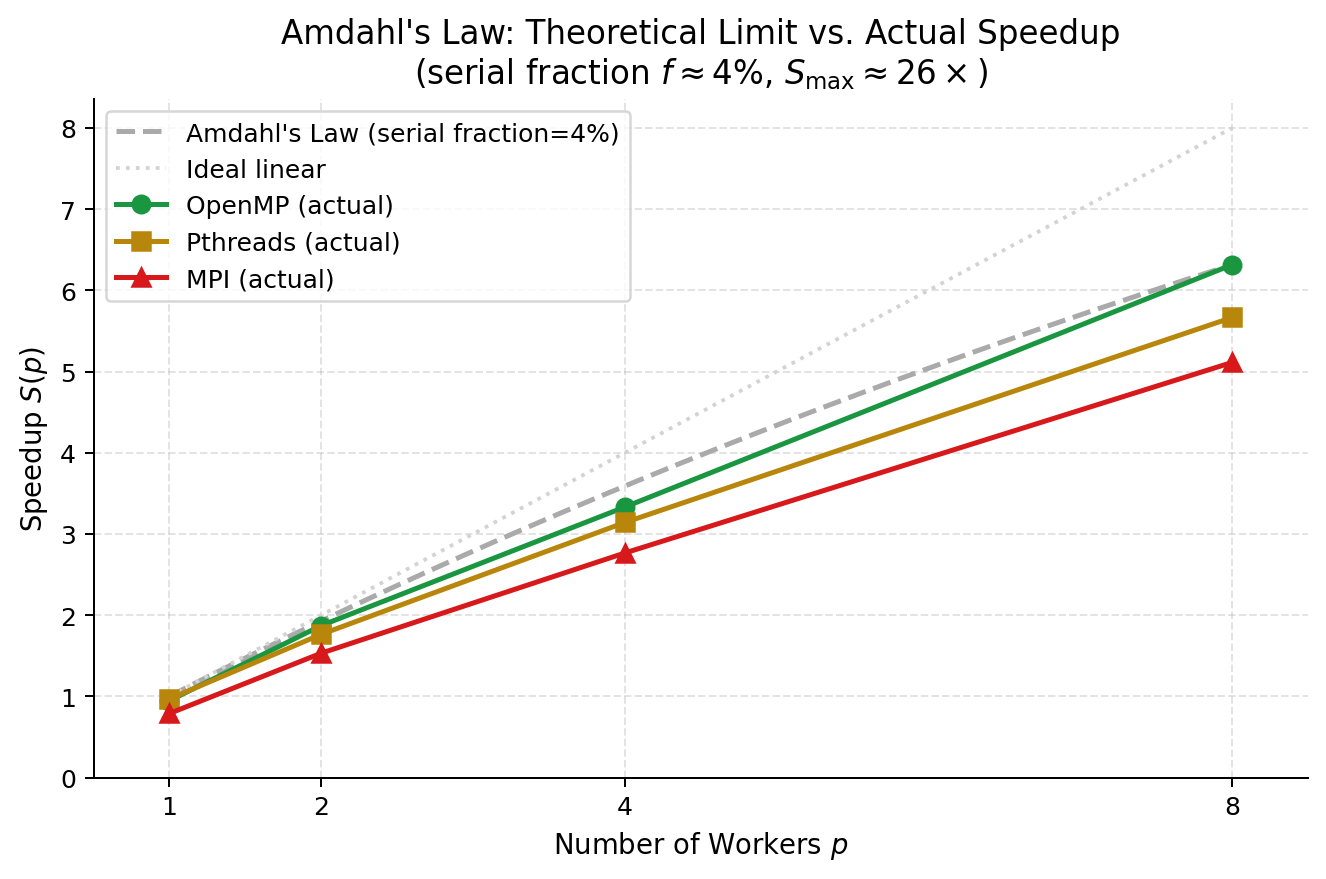
\includegraphics[width=\textwidth]{../analysis_diagrams/charts/amdahls_law.png}
  \caption{Amdahl's Law ($f \approx 4\%$, $S_{\max}\approx25\times$) vs.\ actual speedup.}
\end{figure}

\begin{figure}[H]
  \centering
  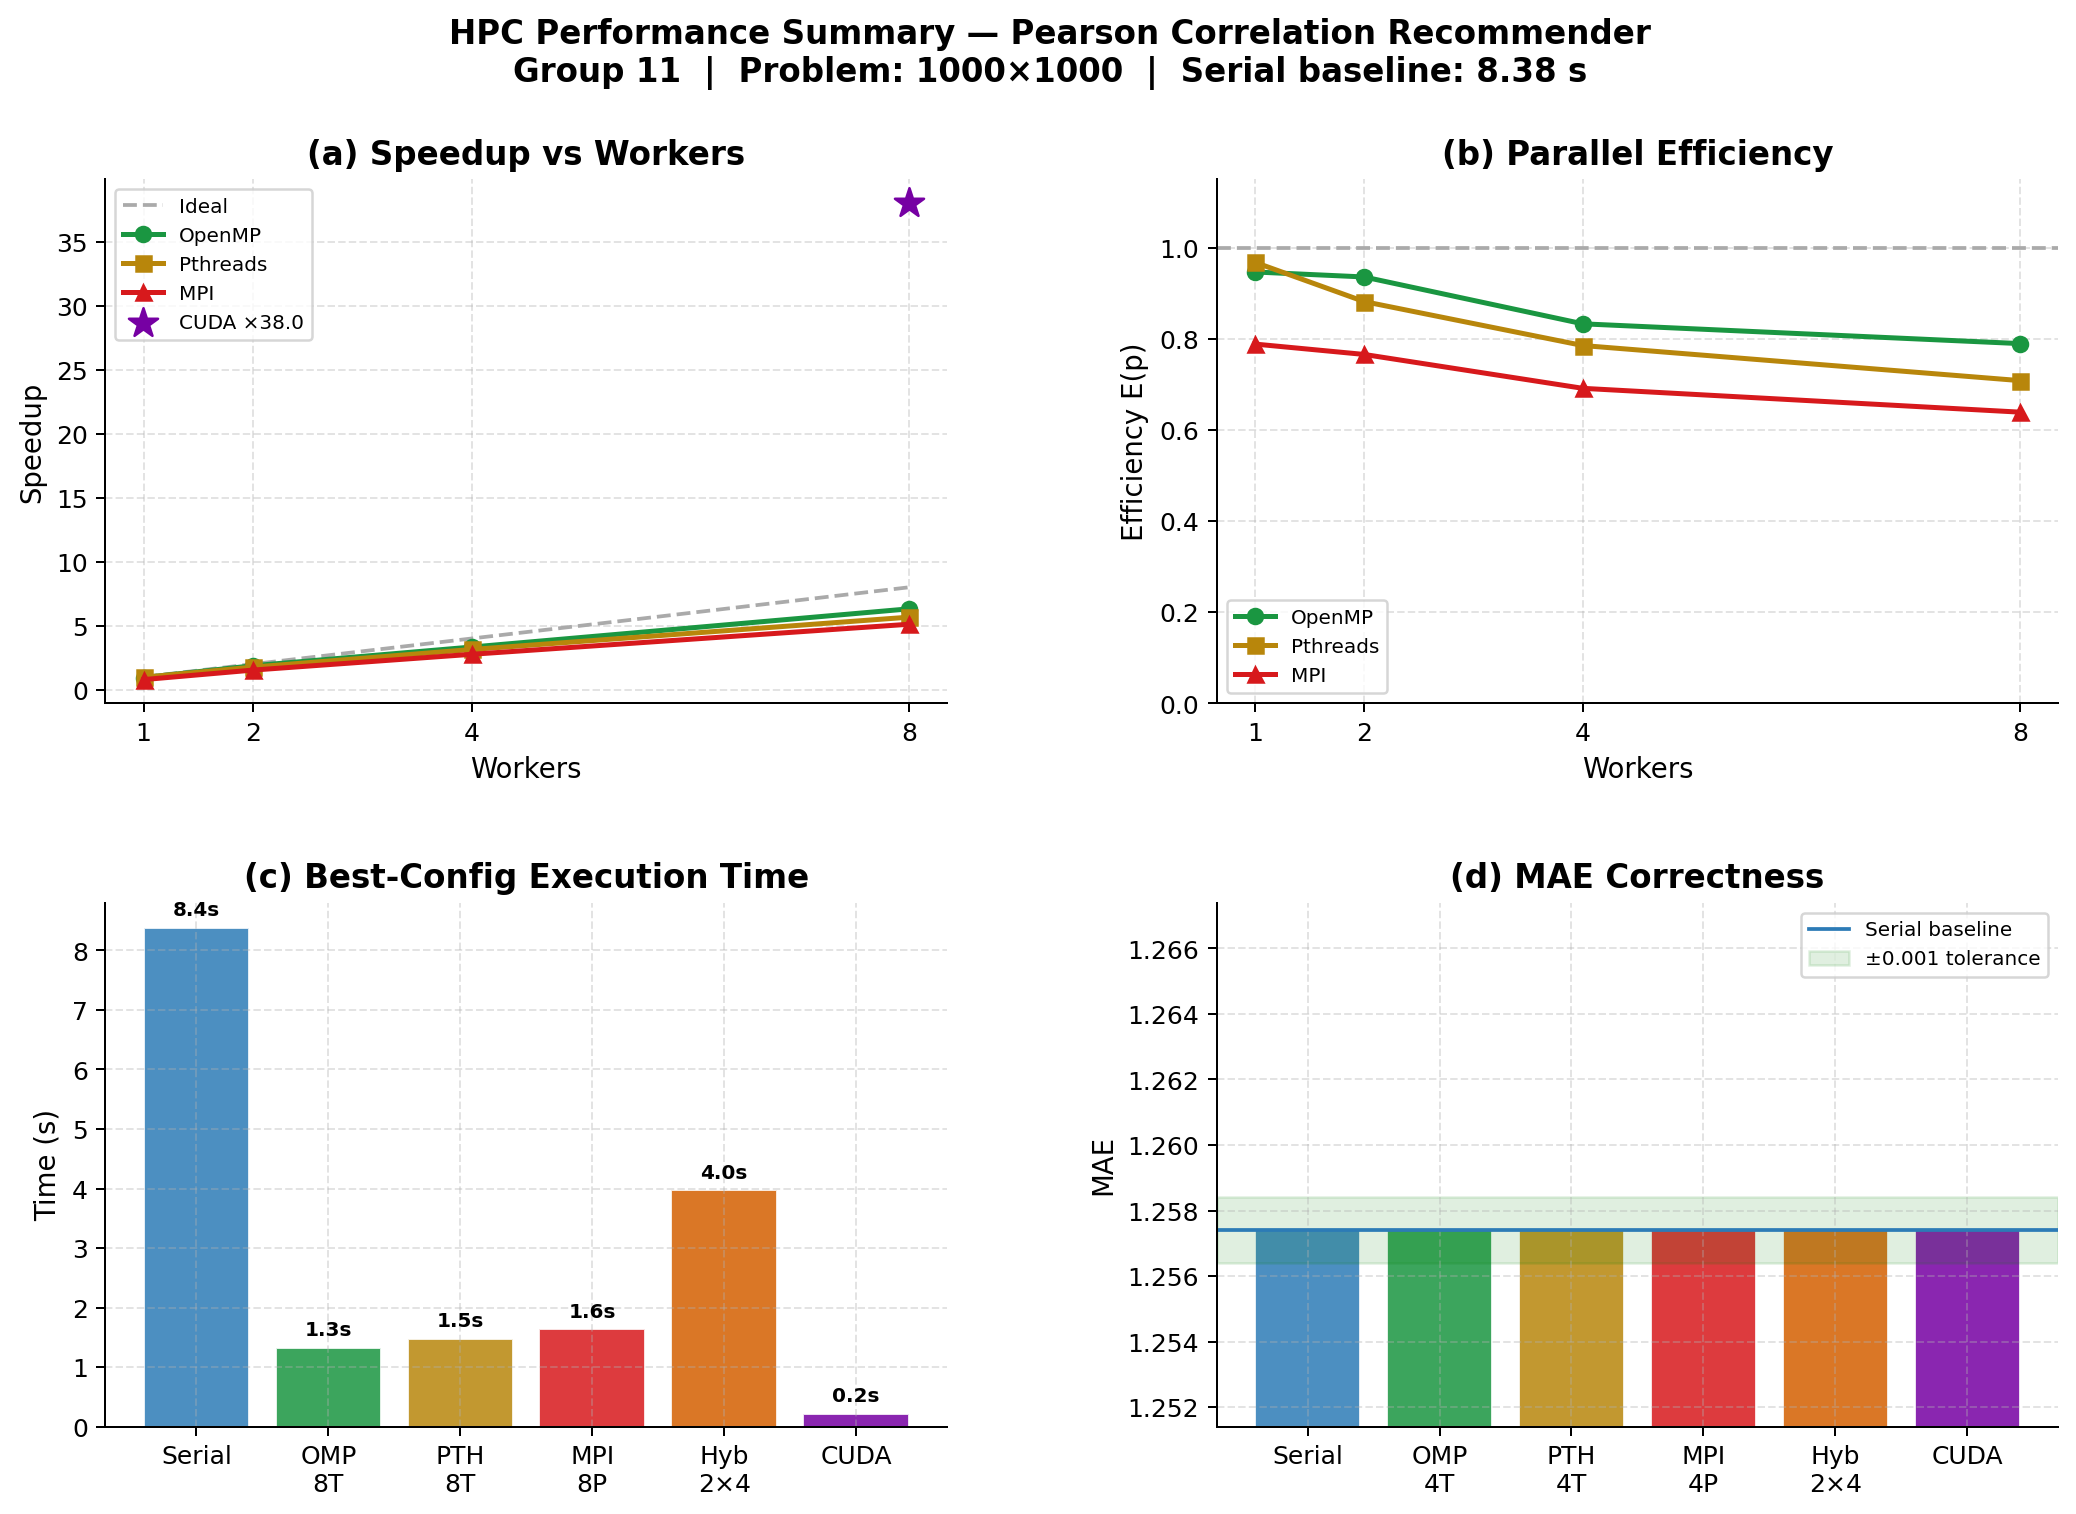
\includegraphics[width=\textwidth]{../analysis_diagrams/charts/summary_dashboard.png}
  \caption{Summary dashboard: (a) speedup, (b) efficiency, (c) execution time, (d) MAE.}
\end{figure}

% ══════════════════════════════════════════════════════════════════════════════
\section{Performance Discussion}
% ══════════════════════════════════════════════════════════════════════════════

\subsection{Head-to-Head Comparison at 8 Workers}

\begin{table}[H]
\centering
\begin{tabular}{L{4cm} R{2.5cm} R{2.5cm} R{2.5cm} R{2.5cm}}
\toprule
\textbf{Version} & \textbf{Total (s)} & \textbf{Speedup} &
\textbf{Efficiency} & \textbf{MAE} \\
\midrule
Serial (baseline)        & 8.3826 & 1.00 & 1.00 & 1.2574 \\
\textbf{CUDA (GPU)}      & \textbf{0.2205} & \textbf{38.02} & --- & 1.2574 \\
OpenMP 8T                & 1.3272 & 6.32 & 0.79 & 1.2574 \\
Pthreads 8T              & 1.4794 & 5.67 & 0.71 & 1.2574 \\
MPI 8P                   & 1.6395 & 5.11 & 0.64 & 1.2574 \\
Hybrid 8$\times$1        & 1.7053 & 4.92 & 0.61 & 1.2574 \\
Hybrid 4$\times$2        & 1.7800 & 4.71 & 0.59 & 1.2574 \\
Hybrid 2$\times$4        & 3.9798 & 2.11 & 0.26 & 1.2574 \\
Hybrid 1$\times$8        & 7.9433 & 1.06 & 0.13 & 1.2574 \\
\bottomrule
\end{tabular}
\caption{Head-to-head: CUDA (GPU) plus all CPU versions at 8 workers. CUDA is the
fastest overall; OpenMP 8T is the best CPU configuration. All MAE values are
identical. (GPU efficiency per-core is not directly comparable, so omitted.)}
\end{table}

\subsection{OpenMP vs.\ Pthreads}

OpenMP ($\times$6.32, 79\% efficiency) outperforms Pthreads ($\times$5.67, 71\%) for three reasons:
\begin{enumerate}
  \item \textbf{Dynamic load balancing:} \code{schedule(dynamic,4)} adapts to the
        triangular loop imbalance.  Static ceiling-division in Pthreads cannot.
  \item \textbf{Thread reuse:} OpenMP reuses threads across Phases 2--4.
        Pthreads creates and joins threads three times per run.
  \item \textbf{Runtime optimisations:} GCC's OpenMP runtime applies
        platform-specific scheduling heuristics.
\end{enumerate}

\subsection{MPI Scaling}

MPI efficiency declines from 79\% ($P=1$) to 64\% ($P=8$).  The
\code{MPI\_Allgatherv} for the $N \times N$ similarity matrix ($\approx 4$\,MB)
limits single-node performance.  At multi-node scale, where shared memory is unavailable, MPI is
the mandatory model and the efficiency gap with OpenMP would be acceptable.

\subsection{Hybrid MPI+OpenMP --- Inversion on a Single Node}

On a single node, more MPI processes yields \emph{better} Hybrid performance:

\begin{center}
Hybrid 8$\times$1 ($\times$4.92) $>$ 4$\times$2 ($\times$4.71)
$>$ 2$\times$4 ($\times$2.11) $>$ 1$\times$8 ($\times$1.06)
\end{center}

When fewer MPI ranks are used, the MPI startup and \code{MPI\_Allgatherv} cost
dominates what is essentially an OpenMP workload.  The Hybrid 1$\times$8
configuration pays all MPI overhead while gaining zero distribution benefit.
\textbf{The Hybrid model's advantage over pure OpenMP only emerges at
multi-node scale.}

\subsection{Amdahl's Law}

\begin{table}[H]
\centering
\begin{tabular}{L{3cm} R{3cm} R{3cm} L{5.5cm}}
\toprule
\textbf{Technology} & \textbf{Predicted} & \textbf{Actual} & \textbf{Observation} \\
\midrule
OpenMP 8T   & 6.25$\times$ & 6.32$\times$ $\uparrow$ &
  Slightly exceeds theory: dynamic scheduling reduces effective $f$ \\
Pthreads 8T & 6.25$\times$ & 5.67$\times$ $\downarrow$ &
  Below theory: static row split cannot balance the triangular load \\
MPI 8P      & 6.25$\times$ & 5.11$\times$ $\downarrow$ &
  Below theory: communication overhead not modelled by Amdahl \\
\bottomrule
\end{tabular}
\caption{Amdahl's Law predictions vs.\ actual measured speedup at $p=8$.}
\end{table}

% ══════════════════════════════════════════════════════════════════════════════
\section{Conclusions}
% ══════════════════════════════════════════════════════════════════════════════

\begin{enumerate}

  \item \textbf{All versions preserve correctness.}  Every
        implementation (CPU and GPU) produces MAE = \textbf{1.2574} and
        checksum = \textbf{942.387323} --- identical to the serial baseline.

  \item \textbf{OpenMP achieves the best CPU performance.}
        $\times$6.32 speedup at 8 threads, 79\% efficiency.  Dynamic scheduling
        and thread reuse explain the advantage.

  \item \textbf{Pthreads is competitive but less efficient.}
        $\times$5.67 at 8T, 71\% efficiency.  Static row assignment and
        per-phase thread creation limit scalability.

  \item \textbf{MPI achieves good speedup with communication overhead.}
        $\times$5.11 at 8P, 64\% efficiency.  MPI would close the gap at
        multi-node scale.

  \item \textbf{Hybrid performance inversely correlates with OpenMP thread count
        on a single node.}  Hybrid 8$\times$1 ($\times$4.92) is the best Hybrid
        configuration; Hybrid 1$\times$8 is the worst ($\times$1.06).  The Hybrid
        advantage over pure OpenMP only emerges at multi-node scale.

  \item \textbf{CUDA provides the largest speedup by far.}  Benchmarked on the
        NVIDIA RTX 3050, the GPU completes similarity + prediction in
        \textbf{0.2205\,s} --- a \textbf{38.0$\times$} speedup over the serial
        baseline and $\approx$6$\times$ faster than the best 8-thread CPU
        run.  The similarity kernel launches 1{,}016{,}064 threads
        simultaneously.

\end{enumerate}

\textbf{Final ranking (single node):}

\begin{center}
CUDA GPU ($\times$38.0)
$>$ OpenMP 8T ($\times$6.32)
$>$ Pthreads 8T ($\times$5.67)
$>$ MPI 8P ($\times$5.11)
$>$ Hybrid 8$\times$1 ($\times$4.92)
$>$ Hybrid 4$\times$2 ($\times$4.71)
$>$ Hybrid 2$\times$4 ($\times$2.11)
$>$ Hybrid 1$\times$8 ($\times$1.06)
\end{center}

% ══════════════════════════════════════════════════════════════════════════════
\section*{References}
% ══════════════════════════════════════════════════════════════════════════════

\begin{enumerate}
  \item J.\ S.\ Breese, D.\ Heckerman, and C.\ Kadie,
        ``Empirical analysis of predictive algorithms for collaborative filtering,''
        \textit{arXiv:1301.7363}, 2013.
  \item B.\ Sarwar, G.\ Karypis, J.\ Konstan, and J.\ Riedl,
        ``Item-based collaborative filtering recommendation algorithms,''
        in \textit{Proc.\ WWW}, pp.\ 285--295, 2001.
  \item B.\ Chapman, G.\ Jost, R.\ van der Pas, \textit{Using OpenMP}. MIT Press, 2008.
  \item W.\ Gropp, E.\ Lusk, A.\ Skjellum, \textit{Using MPI}. MIT Press, 1994.
  \item J.\ Nickolls et al., ``Scalable parallel programming with CUDA,''
        \textit{Queue}, vol.\ 6, no.\ 2, pp.\ 40--53, 2008.
\end{enumerate}

\vfill
\noindent\rule{\linewidth}{0.5pt}\\[0.3em]
{\small Group 11 \quad EC7207 High Performance Computing \quad May 2026}

\end{document}
